\documentclass[twoside,11pt]{report}
% available document structure commands :
% Report: \part{}, \chapter{}, \section{}, \subsection{}, \subsubsection{}, \paragraph{}, \subparagraph{}.

% encoding
\usepackage[utf8]{inputenc}

% maths packages
\usepackage{amsmath}
\usepackage{amssymb}
\usepackage{amsthm}
\usepackage{mathrsfs}
\usepackage{array}
\usepackage{thmtools}
\usepackage{bbm}

% mise en forme
% -------------

% base
% https://www.overleaf.com/learn/latex/Page_size_and_margins
\usepackage[a4paper]{geometry}
% \newgeometry{
%     top=3cm,
%     bottom=3cm,
%     outer=3cm,
%     inner=3cm    
% }
% to have paysage
%  \usepackage{pdflscape}
% paragraph management
% https://mirror.ox.ac.uk/sites/ctan.org/macros/latex/contrib/parskip/parskip.pdf
% spacing management
% https://www.overleaf.com/learn/latex/Articles/How_to_change_paragraph_spacing_in_LaTeX
% \usepackage{parskip}  
% code highlighting
% https://www.overleaf.com/learn/latex/Code_Highlighting_with_minted
% \usepackage{minted}
% draw arrows on side of aligned equations
% https://mirrors.ibiblio.org/CTAN/macros/generic/witharrows/witharrows.pdf
% \usepackage{witharrows}
% graphiques
% https://www.overleaf.com/learn/latex/TikZ_package
\usepackage{tikz} %, pgfplots}
% \pgfplotsset{compat=1.18}
\usetikzlibrary{positioning, arrows.meta}
\usetikzlibrary{bayesnet}
\usetikzlibrary[quotes]
\usetikzlibrary{arrows}
\usetikzlibrary{backgrounds}
\usetikzlibrary{shapes, shapes.geometric, shapes.misc}
% graphicx
% https://fr.overleaf.com/learn/latex/Inserting_Images
\usepackage{graphicx}
\graphicspath{ {./images/figure} }
% verbatim
% https://texdoc.org/serve/fancyvrb/0
\usepackage{fancyvrb}
% headers, footers
% https://www.overleaf.com/learn/latex/Headers_and_footers
\usepackage{fancyhdr}
% chapter headings
% https://texblog.org/2012/07/03/fancy-latex-chapter-styles/
%Options: Sonny, Lenny, Glenn, Conny, Rejne, Bjarne, Bjornstrup
\usepackage[Bjornstrup]{fncychap}
% colors !
% https://fr.overleaf.com/learn/latex/Using_colors_in_LaTeX
\usepackage{color}
\usepackage{xcolor}
% color boxes
% https://www.tug.org/docs/latex/tcolorbox/tcolorbox.pdf
\usepackage{tcolorbox}
\usepackage{xparse}
\tcbuselibrary{theorems, skins, breakable}
%\newtheorem{theorem}{Theorem}[section]
%\newtheorem{definition}{Definition}[section]
% multicolmuns
\usepackage{multicol}
\setlength{\columnsep}{0.5cm}
% package to have text in boxes
\usepackage[]{mdframed}
% glossaries
% https://www.overleaf.com/learn/latex/Glossaries
\usepackage{glossaries}
\makeglossaries
% multicolomuns
\usepackage{multicol}
% algos
\usepackage{algorithm}
\usepackage{algorithmic}
% https://ctan.tetaneutral.net/macros/latex/contrib/titlesec/titlesec.pdf
\usepackage{titlesec}
% appendix and reference
\usepackage[backend=biber,style=ieee,sorting=ynt]{biblatex}
\usepackage[toc,page]{appendix}
% to display tables
\usepackage{booktabs}
% https://fr.wikibooks.org/wiki/LaTeX/Tableaux
% https://ctan.mines-albi.fr/macros/latex/contrib/arydshln/arydshln-man.pdf
\usepackage{tabularx}
\usepackage{arydshln}
% epigraph
\usepackage{epigraph}
% quotes
\usepackage{csquotes}
% to test
\usepackage{lipsum}
% for conditional independence symbol \Perp
\usepackage{txfonts}
% nicer toc
% \usepackage{tocloft}
% \setlength{\cftchapindent}{2em}
% arrows in equations
\usepackage{witharrows}
\usepackage{setspace}
% links
% https://fr.overleaf.com/learn/latex/Hyperlinks
\usepackage[colorlinks=true,urlcolor=blue]{hyperref}
% don't know if useful
% \usepackage{caption}
% \usepackage{subcaption}
\newacronym{dag}{DAG}{Directed Acyclic Graph}
\newacronym{vae}{VAE}{Variational Auto Encoder}
\newacronym{vlb}{VLB}{Variational Lower Bound}
\newacronym{elbo}{ELBO}{Evidence Lower Bound}
\newacronym{dvae}{DVAE}{Dynamical Variational Auto Encoder}
\newacronym{lstm}{LSTM}{Long Short Term Memory}
\newacronym{mlp}{MLP}{Multi Layer Perceptron}
\newacronym{vrnn}{VRNN}{Variational Recurrent Neural Network}
\newacronym{gpm}{GPM}{Graphical Probabilistic Model}
\newacronym{gpvae}{GP-VAE}{Gaussian Process Variational Auto Encoder}
\newacronym{gp}{GP}{Gaussian Process}
\newacronym{sde}{SDE}{Stochastic Differential Equation}
\newacronym{it}{IT}{Information Theory}
\newacronym{apen}{ApEn}{Approximate Entropy}
\newacronym{sampen}{SampEn}{Sample Entropy}
\newacronym{rts}{RTS}{Rauch-Tung-Striebel}
\newacronym{ode}{ODE}{Ordinary Differential Equation}
\newacronym{cd-ssm}{CD-SSM}{Continuous-Discrete State Space Model}
\newacronym{ct-ssm}{CT-SSM}{Continuous-Time State Space Model}
\newacronym{latent-sde}{L-SDE}{Latent Stochastic Differential Equation}
% conditional independence
\newcommand{\indep}{\perp \!\!\! \perp}
\newcommand{\notindep}{\not\!\perp\!\!\!\perp}
\newcommand{\cond}{\, \vert \,}
% real numbers
\newcommand{\R}{\mathbb{R}}
% expectation
\newcommand{\E}[1]{\mathbb{E}_{#1}}
% KL
\newcommand{\KL}[2]{\mathbb{KL}\left( #1 \vert\vert #2 \right)}
% VLB/ELBO
\newcommand{\VLB}{\mathcal{L}(\theta, \phi, X)}
% neural net Gaussian with diagonal covariance
\newcommand{\NNdiag}[3]{\mathcal{N}( #1 \vert #2, \text{diag}\, #3)}
% Brownian motion and related commands
\newcommand{\brownian}{(\Omega, \mathcal{F}, (\mathcal{F}_t)_{t \geq 0}, (B_t)_{t \geq 0}, \mathbb{P})}
\newcommand{\filtration}{(\mathcal{F}_t)_{t \in T}}
\newcommand{\espaceprob}{(\Omega, \mathcal{F}, \mathbb{P})}
\newcommand{\lunomega}{L^1(\Omega, \mathcal{F}, \mathbb{P})}
\newcommand{\ldeuxomega}{L^2(\Omega, \mathcal{F}, \mathbb{P})}
\newcommand{\norm}[1]{\vert \vert #1 \vert \vert}
\input{theorems.tex}

% files for bibliography
% \addbibresource{chapter/references.bib}
\addbibresource{chapter/citations.bib}
\addbibresource{chapter/citations_2.bib}


\title{Dynamical Variational Autoencoders :\\ discrete-time and continuous-time models.\\ Links to stochastic calculus and stochastic differential equations\\
\vspace{2cm}
{\Large{ENS Paris-Saclay, MVA}}}

\author{
Benjamin Deporte : \href{mailto:benjamin.deporte@ens-paris-saclay.fr}{benjamin.deporte@ens-paris-saclay.fr}% student 1
}

\date{August 2025 - DRAFT !}

\begin{document}

\everymath{\displaystyle}
\maketitle

\chapter*{Acknowledgements}

Merci's

\newpage
\singlespacing
\tableofcontents

\newpage
\listoffigures

\part{Introduction}
    
    \chapter{Subject}\label{sec:Subject}

Variational Autoencoders are a well-known class of generative models, where the latent variables are usually assumed to be idependent and identically distributed. This assumption is inappropriate when the data is time-dependent, such as in time-series, images sequences or videos. It is then natural to structure some sort of temporal dependency in the latent prior : this is the main idea of Dynamical VAEs.

A first question is whether the use of Dynamical VAEs on time-dependent data allow better performance than the "legacy" models. A natural test framework is time series, where the usual models -such as ARIMA- have been performing successfully for quite a while.

A second question takes the thinking a little bit deeper. If we consider a time-dependent data sequence as the realization of a stochastic process -which is quite natural for time series, but can be envisioned as well for videos or other sources-, then we infer that some data sequences are, by design, easier than others to predict and learn generative models on. An idea is then to quantity the "randomness" of a data sequence -and more importantly, the "randomness" of the underlying stochastic process-, so we can measure when the use of Dynamical VAEs is likely to add value. A natural tool is Information Theory, where some results exist regarding stochastic processes.

Last but not least, assuming that we have learnt "reasonably well" a generative model, we can wonder how good the model performs at detecting anomalies in the data sequence. The Pandora's box of anomaly detection is vast, and covers connex notions such as detecting outliers in a stationary distribution, detecting shifts of a distribution towards a new one, etc. If using the likelihood of the data according to the learnt distribution is quite straightforward an idea, some recent results show that this may be misleading.
    % \chapter{Report Outline}\label{sec:outline}

\textbf{Part II} covers the mathematical background that is required for most of the report. Section 1 covers the main results regarding stochastic processes and introduces the Brownian motion. (Stochastic Differential Equations are introduced later in Part III). Section 2 recaps the main first definitions and results regarding information theory, its application to stochastic processes, some theoretical results for stationary processes and experimental metrics.

\textbf{Part II} covers discrete-time dynamical Variational AutoEncoders. Section 1 is a recap of graphical models and D-Separation, that is used throughout the report. Section 2 introduces the generic formulation of DVAEs : generative and inference models, variational lower bound. Section 3 presents the first, and most simple model : the Deep Kalman Filter. Section 4 presents the most expressive model, ie the Variationnal RNN. Section 5 is a summary of the take-aways regarding the PyTorch-implementations.

\textbf{Part III} takes us to continuous-time Dynamical VAEs. Section 1 is a recap of the theory regarding Gaussian Processes, that will be at the core of this part. Section 2 is intended to be a self-sustained presentation of the stochastic calculus, where we go quickly over the construction of the Ito's integral to derive the necessary Ito's lemma and subsequent calculation rules for the rest of the report.  Section 3 presents the GP-VAE model. Section 4 is a summary of the take-aways regarding the PyTorch implementation.

\textbf{Part IV} summarizes the experiments : Blembet UK tides, Brownian motion, O.U + Student observation model, cryptos...

\textbf{Part V} is an opening to what could be covered next ! Section 1 presents the link between SDEs and Markovian kernel Gaussian Processes. Section 2 presents some results regarding information theory and stochastic processes.
    % \chapter{Related work}\label{sec:related_work}

\lipsum[1-2]

%
%
%---------------------- DYNAMICAL VAE ---------------------------------------------
%
%
\part{Dynamical Variational Autoencoders}

This part presents the general framework of \glspl{dvae}. We start with a reminder of the key notion of \textbf{D-separation}, which is central in \glspl{gpm}.

Then, we describe three models in details:
\begin{itemize}
    \item \textbf{Deep Kalman Filter} : this model arises as the first evolution of the well-known Kalman Filter, with richer, \glspl{mlp} networks for the encoder and decoder.
    \item \textbf{Variational Recurrent Neural Network} : at the other end of the spectrum, \glspl{vrnn} provide the most expressive discrete-time formulation of the encoder and decoder.
We describe here a different implementation from the one described in \cite{girin_dynamical_2022}.
    \item \textbf{Gaussian Process Variational Auto Encoder} : in this model, the prior over the latent variables is no longer discrete, but is a \gls{gp}.
This allows for sampling data at irregular intervals. Another benefit is the use of richer kernel families to encode prior knowledge.
\end{itemize}

    \chapter{D-separation}\label{sec:D-Separation}

% \section{Graphical Models, Directed Acyclic Graph and factorization of joint probability distributions}
Graphical models are an efficient way to describe families of factorized joint distributions of a data set $(x_i)_{i=1,...,n}$ into a \gls{dag}. 

Given such a dataset, we can build a \gls{dag} where each node is indexed by an integer that is higher than the indexes of its \textit{parent} nodes, such that the joint distribution over the dataset factorizes as:

\begin{align}
p(x_1,x_2,...,x_n) = \prod_{i=1}^n p(x_i \vert pa_i)
\end{align}
where $pa_i$ is the set of parent nodes of $x_i$.\\
For example, the following \gls{dag}

% % --- ORIGINAL : WORKS ----------------------
% \begin{center}
% \begin{tikzpicture}[
%     X/.style={circle, draw=black!80, thin, minimum size=5mm}
% ]
% % nodes
% \node[X] (X1) {$x_1$};
% \node[X] (X2) [right= of X1]{$x_2$} edge [<-, thin] (X1); 
% \node[X] (X3) [below= of X1]{$x_3$} edge [<-, thin] (X1);
% \node[X] (X4) [right= of X3]{$x_4$} edge [<-, thin] (X3)
%                                     edge [<-, thin] (X1);
% \node[X] (X5) [right= of X4]{$x_5$} edge [<-, thin] (X4)
%                                     edge [<-, thin] (X2);
% \end{tikzpicture}
% \end{center}
% describes:
% \begin{align}
%     p(x_1,x_2,x_3,x_4,x_5) &= p(x_1)p(x_2\vert x_1)p(x_3\vert x_1)p(x_4 \vert x_1, x_3)p(x_5 \vert x_2, x_4)
% \end{align}

\begin{center}
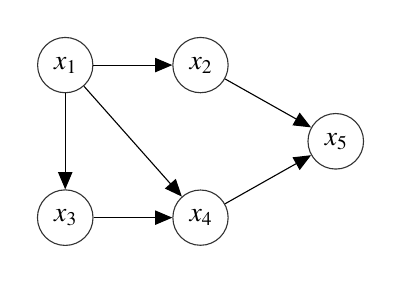
\begin{tikzpicture}[
    X/.style={circle, draw=black!80, thin, minimum size=5mm}
]
% use \matrix to position the nodes
\matrix[row sep=0.25cm, column sep=1cm] {
    % first row
    \node[X] (X1) {$x_1$}; & \node[X] (X2) {$x_2$}; & \\
    & & \node[X] (X5) {$x_5$}; \\
    \node[X] (X3) {$x_3$}; & \node[X] (X4) {$x_4$}; & \\
};
% use \path to draw the edges
\path   (X1) edge[->, thin] (X2)
        (X1) edge[->, thin] (X3)
        (X1) edge[->, thin] (X4)
        (X2) edge[->, thin] (X5)
        (X3) edge[->, thin] (X4)
        (X4) edge[->, thin] (X5);
\end{tikzpicture}
\end{center}
describes:
\begin{align}
    p(x_1,x_2,x_3,x_4,x_5) &= p(x_1)p(x_2\vert x_1)p(x_3\vert x_1)p(x_4 \vert x_1, x_3)p(x_5 \vert x_2, x_4)
\end{align}

% \section{D-separation and conditional independence}

Describing a factorized joint probability distribution by a \gls{dag} allows to determine graphically whether two sets of nodes (ie random variables) are independent, conditioned on a third set of nodes. This allows subsequently to simplify the expressions of the observation models (ie $p(x \vert z)$, and/or the posterior models ($q(z \vert x)$).

\textbf{D-Separation} is the set of rules that determine whether there is conditional independence between two sets given a third one. D-Separation is well described in key books such as \cite{PRML}, \cite{ProbabilisticGraphicalModels} or \cite{ProbabilisticMachineLearning}. We will enunciate here the key concepts, and refer the interested reader to those books.

% \subsection{3-node DAG}

D-Separation is a way to find out graphically conditional (in)dependence relationships between random variables, that would be more difficult to calculate by marginalizing the joint distribution over the conditioning variables. A nice way to demonstrate this, is to review the three examples of 3-node \gls{dag}. 
NB : The observed (ie conditioning) variables are noted with gray background.

% --- EXAMPLE 1 ---------------------------------
\setlength{\columnsep}{1.5cm}
\begin{multicols}{3}[
\textbf{Example 1} : $c$ is said \textit{tail-to-tail} with $a$ and $b$, and \textit{blocks the path between $a$ and $b$}, making them conditionally independent : $a \not\Perp b \cond \varnothing$, $a \Perp b \cond c$
]
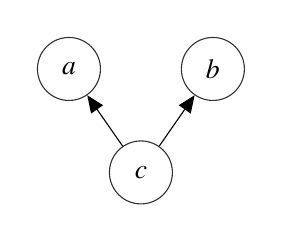
\begin{tikzpicture}[
    UNOBS/.style={circle, draw=black!80, thin, minimum size=8mm},
    OBS/.style={circle, draw=black!80, fill=gray!50, thin, minimum size=8mm}
]
\matrix[row sep=0.5cm, column sep=0.1cm] {
    % first row
    \node[UNOBS] (a) {$a$}; & & \node[UNOBS] (b) {$b$}; & \\
    & \node[UNOBS] (c) {$c$}; & \\
};
\path   (c) edge[->, thin] (b)
        (c) edge[->, thin] (a);
\end{tikzpicture}
% \columnbreak
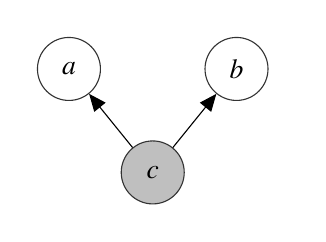
\begin{tikzpicture}[
    UNOBS/.style={circle, draw=black!80, thin, minimum size=8mm},
    OBS/.style={circle, draw=black!80, fill=gray!50, thin, minimum size=8mm}
]
\matrix[row sep=0.5cm, column sep=0.25cm] {
    % first row
    \node[UNOBS] (a) {$a$}; & & \node[UNOBS] (b) {$b$}; & \\
    & \node[OBS] (c) {$c$}; & \\
};
\path   (c) edge[->, thin] (b)
        (c) edge[->, thin] (a);
\end{tikzpicture}
\columnbreak
\begin{align*}
    p(a,b,c) &= p(c)p(a \vert c)p(b \vert c) \\
    p(a,b) &= \sum_c p(c)p(a \vert c)p(b \vert c) \neq p(a)p(b) \\
    &\implies a \not\Perp b \cond \emptyset \\
    p(a,b \vert c) &= p(a \vert c) p(b \vert c) \\
    &\implies a \Perp b \cond c\\
\end{align*}
\end{multicols}


% --- EXAMPLE 2 ---------------------------------
\begin{multicols}{3}[
\textbf{Example 2} : $a,c,b$ form a Markov chain. $c$ is said \textit{head-to-tail} with $a$ and $b$ and, here also, \textit{blocks the path between $a$ and $b$}, making them conditionally independent : $a \notindep b \cond \emptyset$, $a \indep b \vert c$
]
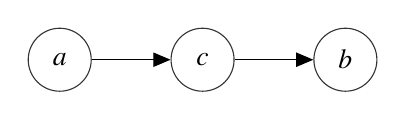
\begin{tikzpicture}[
    UNOBS/.style={circle, draw=black!80, thin, minimum size=8mm},
    OBS/.style={circle, draw=black!80, fill=gray!50, thin, minimum size=8mm}
]
% nodes
\node[UNOBS] (a) {$a$};
\node[UNOBS] (c) [right= of a]{$c$} edge [<-, thin] (a); 
\node[UNOBS] (b) [right= of c]{$b$} edge [<-, thin] (c);
\end{tikzpicture}
% \columnbreak
\vspace{2cm}
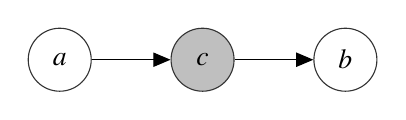
\begin{tikzpicture}[
    UNOBS/.style={circle, draw=black!80, thin, minimum size=8mm},
    OBS/.style={circle, draw=black!80, fill=gray!50, thin, minimum size=8mm}
]
% nodes
\node[UNOBS] (a) {$a$};
\node[OBS] (c) [right= of a]{$c$} edge [<-, thin] (a); 
\node[UNOBS] (b) [right= of c]{$b$} edge [<-, thin] (c);
\end{tikzpicture}
\columnbreak
\begin{align*}
    p(a,b,c) &= p(a)p(c \vert a) p(b \vert c) \\
    p(a,b) &\neq p(a)p(b) \implies a \not\Perp b \vert \emptyset \\
    p(a,b \vert c) &= \frac{p(a)p(c \vert a)}{p(c)}p(b \vert c) = p(a \vert c) p(b \vert c) \implies a \Perp b \cond c\\
\end{align*}
\end{multicols}

% --- EXAMPLE 3 ---------------------------------
\setlength{\columnsep}{1.5cm}
\begin{multicols}{3}[
\textbf{Example 3} : $c$ is said \textit{head-to-head} with $a$ and $b$. In this head-to-head configuration, contrary to the two examples above, \textit{the path between $a$ and $b$ is blocked when $c$ is unobserved} : $a \Perp b \cond \emptyset$, $a \not\Perp b \cond c$
]
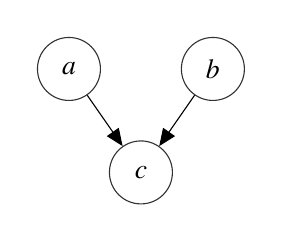
\begin{tikzpicture}[
    UNOBS/.style={circle, draw=black!80, thin, minimum size=8mm},
    OBS/.style={circle, draw=black!80, fill=gray!50, thin, minimum size=8mm}
]
\matrix[row sep=0.5cm, column sep=0.1cm] {
    % first row
    \node[UNOBS] (a) {$a$}; & & \node[UNOBS] (b) {$b$}; & \\
    & \node[UNOBS] (c) {$c$}; & \\
};
\path   (c) edge[<-, thin] (b)
        (c) edge[<-, thin] (a);
\end{tikzpicture}
% \columnbreak
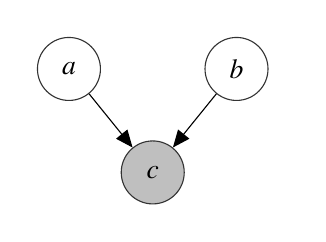
\begin{tikzpicture}[
    UNOBS/.style={circle, draw=black!80, thin, minimum size=8mm},
    OBS/.style={circle, draw=black!80, fill=gray!50, thin, minimum size=8mm}
]
\matrix[row sep=0.5cm, column sep=0.25cm] {
    % first row
    \node[UNOBS] (a) {$a$}; & & \node[UNOBS] (b) {$b$}; & \\
    & \node[OBS] (c) {$c$}; & \\
};
\path   (c) edge[<-, thin] (b)
        (c) edge[<-, thin] (a);
\end{tikzpicture}
\columnbreak
\begin{align*}
    p(a,b,c) &= p(a)p(b)p(c \vert a, b) \\
    p(a,b) &= \sum_c p(a)p(b)p(c \vert a, b) = p(a)p(b) \\ &\implies a \Perp b \cond \emptyset \\
    p(a,b \vert c) &\neq p(a \vert c) p(b \vert c) \\ &\implies a \not\Perp b \cond c\\
\end{align*}
\end{multicols}

% \subsection{General D-Separation theorem}

We can extend the notion to full sets of nodes.

\begin{tcolorbox}[colback=blue!5!white,colframe=black!75!black,title=D-Separation]
    Let $\mathcal{G}$ be a \gls{dag}.
    
    Let $A, B, C$ three disjoint sets of nodes in $\mathcal{G}$ : $A \cap B = A \cap C = B \cap C = \emptyset$. 
    
    $C$ is the set of "conditioning nodes", or "observed variables".

    We aim to determine whether $A \Perp B \cond C$.

    \textbf{Algorithm}
    \begin{enumerate}
        \item \textbf{Evaluate each path between $A$ and $B$}
        
        Evaluate each possible path between any point $a \in A$, and any point $b \in B$. Such a path between $a$ and $b$ is said \textbf {blocked} if it contains one node $n$ such that one of two following conditions is true:
        
            \begin{itemize}
                \item arrows in the path are \textit{head-to-tail} or \textit{tail-to-tail} at node $n$, and $n \in C$ ($n$ is an observed/conditioning node).
                \item arrows in the path are \textit{head-to-head} at node $n$, and $n \notin C$ and none of $n$ descendants is in $C$
            \end{itemize}
            
        \item \textbf{Assess all paths}
            \begin{itemize}
                \item If all paths $(a,b), a \in A, b \in B$ are blocked, then $A$ is said \textbf{D-separated} from $B$ by $C$, and the joint distribution defined by $\mathcal{G}$ verifies $A \Perp B \cond C$.
                \item If there is at least one path $(a,b), a \in A, b \in B$ that is not blocked then $A \not\Perp B \cond C$.
            \end{itemize}
    \end{enumerate}
\end{tcolorbox}
    \chapter{Dynamical Variational Auto Encoders}\label{sec:DVAEs}

\gls{vae} models are well known and documented (see for example the seminal paper \cite{kingma_introduction_2019}. (A self-contained brief summary of \gls{vae} can be found in appendix \ref{Vanilla VAE}). 

When dealing with sequential data, the i.i.d assumption on latent variables $z_i$ is a limitation. By D-separation, all $x_i$'s are independent of each other conditionally by $z_i$ : $p(x_i \vert x_1, x_2,...,x_{i-1},x_{i+1},..,x_n,z_i) = p(x_i \vert z_i)$. Therefore, a vanilla VAE can not account for correlations between $x_i$ across time.

\glspl{dvae} encode a temporal dependency in the latent variables prior distribution. In this chapter, we review the general discrete-time setting, where the latent variables are countable and indexed by time. An exhaustive review of discrete-time \glspl{dvae} can be found in \cite{girin_dynamical_2022}.

We start by some notations.

\begin{tcolorbox}[colback=blue!5!white,colframe=black!75!black,title=Notations]
\begin{itemize}
    \item the data is a sequence of $T$ points noted \textbf{$x_{1:T}$} $= \{(x_t)_{t=1,...,T}\} \in \mathbb{R}^F$.
    \item the sequence of the associated $T$ latent variables is \textbf{$z_{1:T}$} $= \{(z_t)_{t=1,...,T}\} \in \mathbb{R}^L$
    \item optionally, there may be a sequence of -usually deterministic- $T$ inputs $u_{1:T} = \{(u_t)_{t=1,...,T}\} \in \mathbb{R}^U$
\end{itemize}
\end{tcolorbox}

The generative model is given by the general expression of the joint distribution (here with a sequence of inputs) $p(x_{1:T}, z_{1:T} \vert u_{1:T})$:

\begin{align*}
    p(x_{1:T}, z_{1:T} \vert u_{1:T}) &= \prod_{t=1}^T p(x_t, z_t \vert x_{1:t-1}, z_{1:t-1}, u_{1:T}) \\
    &= \prod_{t=1}^T p(x_t \vert x_{1:t-1}, z_{1:t}, u_{1:T}) p(z_t \vert x_{1:t-1}, z_{1:t-1}, u_{1:T}) \\
    &= \prod_{t=1}^T p(x_t \vert x_{1:t-1}, z_{1:t}, u_{1:t}) p(z_t \vert x_{1:t-1}, z_{1:t-1}, u_{1:t})
\end{align*}

where the only assumption that is made is a causal dependency of the $x_t, z_t$ on the inputs $u_{1:t}$, thus allowing to change the conditioning $\vert u_{1:T}$ into $\vert u_{1:t}$

In the rest of the report, we will consider systems with no input, and drop the conditioning on $u_{1:t}$ to simplify notations. However, the reasoning remains the same with inputs.

The true posterior  $p(z_{1:T} \vert x_{1:T})$ is usually untractable, but can be developed:
\begin{align*}
    p(z_{1:T} \vert x_{1:T}) &= \prod_{t=1}^T p(z_t \vert z_{1:t-1}, x_{1:T})
\end{align*}

It can be noted that the true posterior exhibits a dependence of $z_t$ on \textit{past} $z_{1:t-1}$, but a dependence on the \textit{whole} data sequence $x_{1:T}$ (think Kalman smoother).

As in vanilla \glspl{vae}, the inference model is the approximation of the true posterior by an parametric encoder $q_{\phi}(z_{1:T} \vert x_{1:T})$, where $\phi$ is the set of parameters:
\begin{align*}
    q_{\phi}(z_{1:T} \vert x_{1:T}) &= \prod_{t=1}^T q_\phi(z_t \vert z_{1:t-1}, x_{1:T})
\end{align*}

Depending on the chosen graphical models and the corresponding D-separation results, the observation model $p_{\theta_x}(x_t \vert x_{1:t-1}, z_{1:t}, u_{1:t})$ (with $\theta_x$ the set of parameters of the observation model) and approximate posterior $q_\phi(z_t \vert z_{1:t-1}, x_{1:T})$ may simplify. 

It is also considered a good practice (\cite{girin_dynamical_2022}) to copy/paste the expression of $q_\phi(z_t \vert z_{1:t-1}, x_{1:T})$ from the expression of the true posterior resulting from the D-separation analysis (see next chapters for examples).

Equipped with the generative model and the inference model, we compute the log likelihood of the data $x_{1:T}$ and derive an \gls{vlb} for training (using the same manipulation as for vanilla \gls{vae} : multiplying both sides of the equation by $q_\phi$ and integrating over $dz_{1:T}$)
\begin{align}
    \log{p(x_{1:T})} &= \log{\frac{p(x_{1:T}, z_{1:T})}{p(z_{1:T} \vert x_{1:T})}} \\
    &= \E{q_{\phi}(z_{1:T}\vert x_{1:T})} \log{\frac{p(x_{1:T}, z_{1:T})}{q_{\phi}(z_{1:T}\vert x_{1:T})} \frac{q_{\phi}(z_{1:T}\vert x_{1:T})}{p(z_{1:T} \vert x_{1:T})}} \\
    &= \E{q_{\phi}(z_{1:T}\vert x_{1:T})} \log{\frac{p(x_{1:T}, z_{1:T})}{q_{\phi}(z_{1:T}\vert x_{1:T})} + \KL{q_{\phi}(z_{1:T}\vert x_{1:T})}{p(z_{1:T} \vert x_{1:T})}} \\
    &\geq \E{q_{\phi}(z_{1:T}\vert x_{1:T})} \log{\frac{p(x_{1:T}, z_{1:T})}{q_{\phi}(z_{1:T}\vert x_{1:T})}} = \VLB
\end{align}

The dependence of $\VLB$ on $\theta$ is made more obvious when developing $\VLB$.

Remember we have (making the set of parameters explicit) :
\begin{align}
    p_{\theta}(x_{1:T}, z_{1:T}) &= \prod_{t=1}^T p_{\theta_x}(x_t \vert x_{1:t-1}, z_{1:t}) p_{\theta_z}(z_t \vert z_{1:t-1}, x_{1:t-1}) \\
    \label{q_phi_dev}
    q_\phi(z_{1:T} \vert x_{1:T}) &= \prod_{t=1}^T q_\phi (z_t \vert z_{1:t-1}, x_{1:T})
\end{align}
Therefore
\begin{align}
    \VLB &= \E{q_{\phi}(z_{1:T}\vert x_{1:T})} \log{\left( \frac{\prod_{t=1}^T p_{\theta_x}(x_t \vert x_{1:t-1}, z_{1:t}) p_{\theta_z}(z_t \vert z_{1:t-1}, x_{1:t-1})}{\prod_{t=1}^T q_\phi (z_t \vert z_{1:t-1}, x_{1:T})} \right)} \\
    &= \E{q_{\phi}(z_{1:T}\vert x_{1:T})} \left(  \sum_{t=1}^T \log{p_{\theta_x}(x_t \vert x_{1:t-1}, z_{1:t})} - \sum_{t=1}^T \log{\frac{q_\phi (z_t \vert z_{1:t-1}, x_{1:T})}{p_{\theta_z}(z_t \vert z_{1:t-1}, x_{1:t-1})}}
    \right)
\end{align}

At this point, the expectations require some work. First, we note that, as $q_\phi$ develops as \ref{q_phi_dev}, for any function $\Psi$, the first expectation can be written (note the change in indexes of $z$)
\begin{align*}
    \E{q_{\phi}(z_{1:T}\vert x_{1:T})} \Psi(z_{1:t}) &= \E{q_\phi(z_{1:t} \vert x_{1:T})}\Psi(z_{1:t})
\end{align*}

Second, we develop further and write:
\begin{align*}
    \E{q_{\phi}(z_{1:T}\vert x_{1:T})} \Psi(z_{1:t}) &= \E{q_\phi(z_{1:t} \vert x_{1:T})}\Psi(z_{1:t}) \\
    &= \E{q_\phi(z_{1:t-1} \vert x_{1:T})} \E{q_\phi(z_t \vert z_{1:t-1}, x_{1:T})} \Psi(z_{1:t})
\end{align*}
Therefore the \gls{vlb} becomes:
\begin{align}
    \VLB &= \E{q_\phi(z_{1:t} \vert x_{1:T})}\sum_{t=1}^T \log{p_{\theta_x}(x_t \vert x_{1:t-1}, z_{1:t})} - \sum_{t=1}^T \E{q_\phi(z_{1:t-1} \vert x_{1:T})} \left[ \E{q_\phi(z_t \vert z_{1:t-1}, x_{1:T})} \log{\frac{q_\phi(z_t \vert z_{1:t-1}, x_{1:T})}{p_{\theta_z}(z_t \vert z_{1:t-1}, x_{1:t-1})}}\right] \\
    &= \sum_{t=1}^T \E{q_\phi(z_{1:t} \vert x_{1:T})} \log{p_{\theta_x}(x_t \vert x_{1:t-1}, z_{1:t})} - \sum_{t=1}^T \E{q_\phi(z_{1:t-1} \vert x_{1:T})} \KL{q_\phi(z_t \vert z_{1:t-1}, x_{1:T})}{p_{\theta_z}(z_t \vert z_{1:t-1}, x_{1:t-1})}
\end{align}

As for the vanilla \gls{vae}, the \gls{vlb} contains two terms.

\begin{itemize}
    \item The first term is the reconstruction error. it is the sum over the time steps, of the average log likelihood the data at time $t$, given the approximate distribution of the past and present latent variables, and the past data.
    \item The second term is a regularization term, summing over the time steps the average divergence between the approximate posterior distribution of the latent variable at time $t$, and its real distribution.
\end{itemize}

As in vanilla \gls{vae}, the sampling over $q_\phi$ requires the use of the "re parametrization trick" (see \cite{kingma_introduction_2019}), for $\VLB$ to be differentiable w.r.t. $\theta, \phi$.

Here is the summary regarding \gls{dvae}:

\begin{tcolorbox}[colback=blue!5!white,colframe=black!75!black,title=General Dynamical VAEs]
\begin{itemize}
    \item \textbf{generative model}
    \begin{align}
        \label{gen_model_dvae}
        p(x_{1:T}, z_{1:T}) &= \prod_{t=1}^T p_{\theta_x} (x_t \vert x_{1:t-1}, z_{1:t}) p_{\theta_z}(z_t \vert z_{1:t-1}, x_{1:t-1})
    \end{align}
    \item \textbf{inference model}
    \begin{align}
        \label{inf_model_dvae}
        q_{\phi}(z_{1:T} \vert x_{1:T}) &= \prod_{t=1}^T q_\phi(z_t \vert z_{1:t-1}, x_{1:T})
    \end{align}
    \item \textbf{\gls{vlb} for training}
    \begin{align}
        \label{vlb_dvae}
        \begin{split}
         \VLB &= \sum_{t=1}^T \E{q_\phi(z_{1:t} \vert x_{1:T})} \log{p_{\theta_x}(x_t \vert x_{1:t-1}, z_{1:t})} \\ &- \sum_{t=1}^T \E{q_\phi(z_{1:t-1} \vert x_{1:T})} \KL{q_\phi(z_t \vert z_{1:t-1}, x_{1:T})}{p_{\theta_z}(z_t \vert z_{1:t-1}, x_{1:t-1})}
         \end{split}
    \end{align}
\end{itemize}
\end{tcolorbox}
    \chapter{Deep Kalman Filter}\label{sec:DKF}

The Kalman Filter is a well known model, widely used to denoise time series observations and make predictions. The latent variables form a Markov Chain, and all the probability distributions (ie encoder, decoder and transition model) are linear Gaussians. This allows to derive close form expressions for the solutions (Kalman filter and Kalman smoother).

In a \textbf{Deep Kalman Filter}, the temporal structure of the latent variables is still a Markov Chain. The probaility models are still Gaussians, but with parameters mean and covariance learnt by neural networks.

More specifically, the \gls{dag} describing a Deep Kalman Filter is:

\begin{figure}[h]
    \centering
    % \includegraphics[width=0.5\linewidth]{}
    \label{fig:graphical_model_dkf}
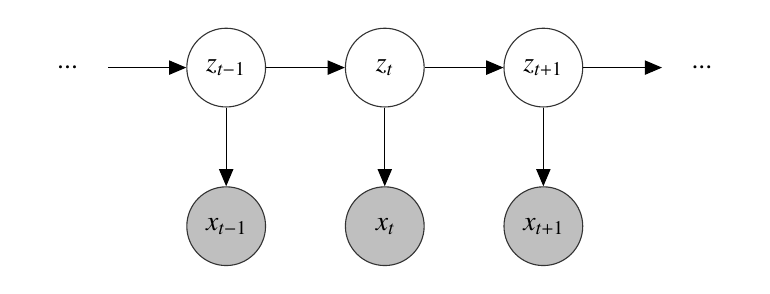
\begin{tikzpicture}[
    HIDDEN/.style={circle, draw=black!0, thin, minimum size=10mm},
    UNOBS/.style={circle, draw=black!80, thin, minimum size=10mm},
    OBS/.style={circle, draw=black!80, fill=gray!50, thin, minimum size=10mm}
]
% nodes
\node[HIDDEN] (a) {$...$};
\node[UNOBS] (z_t_1) [right= of a] {$z_{t-1}$} edge[<-, thin] (a);
\node[UNOBS] (z_t)  [right= of z_t_1] {$z_{t}$} edge[<-, thin] (z_t_1);
\node[UNOBS] (z_t_p1) [right= of z_t] {$z_{t+1}$} edge[<-, thin] (z_t);
\node[HIDDEN] (e) [right= of z_t_p1] {$...$} edge[<-, thin] (z_t_p1);
\node[OBS] (x_t_1) [below= of z_t_1] {$x_{t-1}$} edge[<-, thin] (z_t_1);
\node[OBS] (x_t) [below= of z_t] {$x_{t}$} edge[<-, thin] (z_t);
\node[OBS] (x_t_p1) [below= of z_t_p1] {$x_{t+1}$} edge[<-, thin] (z_t_p1);
\end{tikzpicture}
\caption{Probabilistic model of a Deep Kalman Filter}
\end{figure}

It is then particularly useful to use D-separation on the \gls{dag} to simplify the general \gls{dvae} expressions \ref{gen_model_dvae} and \ref{inf_model_dvae}. Conditioning on $z_t$ and $z_{t-1}$ drives:
\begin{align}
    p_{\theta_x}(x_t \vert x_{1:t-1}, z_{1:t}) &= p_{\theta_x}(x_t \vert z_t) \\
    p_{\theta_z}(z_t \vert z_{1:t-1}, x_{1:t}) &= p_{\theta_z}(z_t \vert z_{t-1}) \\
    \label{dkf_posterior}
    q_{\phi}(z_t \vert z_{1:t-1}, x_{1:T}) &= q_{\phi}(z_t \vert z_{t-1}, x_{t:T}) 
\end{align}

We then choose Gaussian distributions for $p_{\theta_x}, p_{\theta_z}$ and $q_\phi$, with mean and diagonal covariance, learnt by neural networks.
\begin{align}
    p_{\theta_x}(x_t \vert z_t) &= \NNdiag{x_t}{\mu_{\theta_x}(z_t)}{\sigma_{\theta_x}^2(z_t)}\\
    p_{\theta_z}(z_t \vert z_{t-1}) &= \NNdiag{z_t}{\mu_{\theta_z}(z_{t-1})}{\sigma_{\theta_z}^2(z_{t-1})}\\
    q_{\phi}(z_t \vert z_{t-1}, x_{t:T}) &= \NNdiag{z_t}{\mu_{\phi}(z_{t-1}, x_{t:T})}{\sigma_{\theta_z}^2(z_{t-1},x_{t:T})}
\end{align}
Some other formulations of the approximate posterior (encoder) are possible. For example:
\begin{align*}
    q_{\phi}(z_t \vert z_{t-1}, x_t) \\
    q_{\phi}(z_t \vert z_{1:t}, x_{1:t}) \\
    q_{\phi}(z_t \vert z_{1:T}, x_{1:T})
\end{align*}
We have chosen \ref{dkf_posterior} for the implementation, as it has the same formulation as the true posterior and respects the corresponding dependencies.

Taking note that:
\begin{align*}
    q_{\phi}(z_{1:t} \vert x_{1:T}) = q_{\phi}(z_{1:t-1} \vert z_t, x_{1:T}) q_{\phi}(z_t \vert x_{1:T})
\end{align*}
And using D-Separation, the \gls{elbo} \ref{vlb_dvae} simplifies into:
\begin{align}
    \VLB &= \sum_{t=1}^T \E{q_\phi(z_{1:t} \vert x_{1:T})} \log{p_{\theta_x}(x_t \vert z_t)} - \sum_{t=1}^T \E{q_\phi(z_{1:t-1} \vert x_{1:T})} \KL{q_{\phi}(z_t \vert z_{t-1}, x_{t:T})}{p_{\theta_z}(z_t \vert z_{t-1})} \\
    &= \sum_{t=1}^T \E{q_\phi(z_{t} \vert x_{1:T})} \log{p_{\theta_x}(x_t \vert z_t)} - \sum_{t=1}^T \E{q_\phi(z_{t-1} \vert x_{1:T})} \KL{q_{\phi}(z_t \vert z_{t-1}, x_{t:T})}{p_{\theta_z}(z_t \vert z_{t-1})}
\end{align}

As a summary:
\begin{tcolorbox}[colback=blue!5!white,colframe=black!75!black,title=Deep Kalman Filter]
\begin{itemize}
    \item \textbf{generative model}
    \begin{align}
        \label{gen_model_dkf}
        p_{\theta_x}(x_t \vert z_t) &= \NNdiag{x_t}{\mu_{\theta_x}(z_t)}{\sigma_{\theta_x}^2(z_t)}\\
        p_{\theta_z}(z_t \vert z_{t-1}) &= \NNdiag{z_t}{\mu_{\theta_z}(z_{t-1})}{\sigma_{\theta_z}^2(z_{t-1})}
    \end{align}
    \item \textbf{inference model}
    \begin{align}
        \label{inf_model_dkf}
        q_{\phi}(z_t \vert z_{t-1}, x_{t:T}) &= \NNdiag{z_t}{\mu_{\phi}(z_{t-1}, x_{t:T})}{\sigma_{\theta_z}^2(z_{t-1},x_{t:T})}
    \end{align}
    \item \textbf{\gls{vlb} for training}
    \begin{align}
        \label{vlb_dkf}
        \VLB &= \sum_{t=1}^T \E{q_\phi(z_{t} \vert x_{1:T})} \log{p_{\theta_x}(x_t \vert z_t)} - \sum_{t=1}^T \E{q_\phi(z_{t-1} \vert x_{1:T})} \KL{q_{\phi}(z_t \vert z_{t-1}, x_{t:T})}{p_{\theta_z}(z_t \vert z_{t-1})}
    \end{align}
\end{itemize}
\end{tcolorbox}

The $\KL{q_\phi}{p_{\theta_z}}$'s have a close form, as the two distributions are Gaussians.

From a code stand-point, following \cite{girin_dynamical_2022}, we have used forward \gls{lstm} to encode sequences such as $x_{1:t}$, and backward \gls{lstm} to encode sequences such as $x_{t:T}$, as inputs into the \gls{mlp} parametrizing the distributions. 

For example:
\begin{align*}
    \overleftarrow{g_t} &= \text{Backward LSTM}(\overleftarrow{g_{t+1}}, x_t) \,\, (\text{encodes} \,\, x_{t:T}) \\
    q_{\phi}(z_t \vert z_{t-1}, x_{t:T}) &= \NNdiag{z_t}{\mu_{\phi}(z_{t-1}, \overleftarrow{g_t})}{\sigma_{\phi}^2(z_{t-1}, \overleftarrow{g_t})}
\end{align*}



The PyTorch implementation recipes and tricks are described in a subsequent chapter.
    \chapter{Variational Recurrent Neural Network}\label{sec:VRNN}

The \gls{vrnn} is the most expressive \gls{dvae}, in that sense that the general expressions \ref{gen_model_dvae}, \ref{inf_model_dvae} and \gls{vlb} \ref{vlb_dvae} can not be simplified.

The \gls{gpm} of the \gls{vrnn} assumes full connections between latent variables, and between observed variables, to account for the full unsimplified expressions. Specifically:

\begin{figure}[h]
    \centering
    % \includegraphics[width=0.5\linewidth]{}
    \label{fig:graphical_model_vrnn}
\begin{tikzpicture}[
    HIDDEN/.style={circle, draw=black!0, thin, minimum size=10mm},
    UNOBS/.style={circle, draw=black!80, thin, minimum size=10mm},
    OBS/.style={circle, draw=black!80, fill=gray!50, thin, minimum size=10mm}
]
% nodes
\node[HIDDEN] (zs) {$...$}; % start z
\node[HIDDEN] (xs) [below= of zs] {$...$}; % start x
\node[UNOBS] (z_t_1) [right= of zs] {$z_{t-1}$} edge[<-, thin] (a);
\node[OBS] (x_t_1) [below= of z_t_1] {$x_{t-1}$}    edge[<-, thin] (z_t_1)
                                                    edge[<-, thin] (xs);
\node[UNOBS] (z_t)  [right= of z_t_1] {$z_{t}$} edge[<-, thin] (z_t_1)
                                                edge[<-, thin] (x_t_1);
\node[OBS] (x_t) [below= of z_t] {$x_{t}$}  edge[<-, thin] (z_t)
                                            edge[<-, thin] (x_t_1)
                                            edge[<-, thin] (z_t_1);
\node[UNOBS] (z_t_p1) [right= of z_t] {$z_{t+1}$}   edge[<-, thin] (z_t)
                                                    edge[<-, thin] (x_t);
\node[OBS] (x_t_p1) [below= of z_t_p1] {$x_{t+1}$}  edge[<-, thin] (z_t_p1)
                                                    edge[<-, thin] (x_t)
                                                    edge[<-, thin] (z_t);
\node[HIDDEN] (ze) [right= of z_t_p1] {$...$} edge[<-, thin] (z_t_p1); % end z
\node[HIDDEN] (xe) [right= of x_t_p1] {$...$} edge[<-, thin] (x_t_p1); % end x

\path[->]   (z_t_1) edge [bend left=+45] node[mid left] {} (z_t_p1)
            (x_t_1) edge [bend left=-45] node[mid left] {} (x_t_p1);
\end{tikzpicture}
\caption{Probabilistic model of a Variational RNN}
\end{figure}

We remember that:
\begin{align*}
    p(x_{1:T}, z_{1:T}) &= \prod_{t=1}^T p_{\theta_x}(x_t \vert x_{1:t-1}, z_{1:t}) p_{\theta_z}(z_t \vert x_{1:t-1}, z_{1:t-1})
\end{align*}

And posit Gaussian distributions with diagonal covariance and mean given by two networks:
\begin{align}
    p_{\theta_x}(x_t \vert x_{1:t-1}, z_{1:t}) &= \NNdiag{x_t}{\mu_{\theta_x}(x_{1:t-1}, z_{1:t})}{\sigma_{\theta_x}^2(x_{1:t-1}, z_{1:t})} \\
    p_{\theta_z}(z_t \vert z_{1:t-1}, x_{1:t-1}) &= \NNdiag{z_t}{\mu_{\theta_z}(z_{1:t-1}, x_{1:t-1})}{\sigma_{\theta_z}^2(z_{1:t-1}, x_{1:t-1})}
\end{align}

The true posterior being
\begin{align*}
    p(z_{1:T} \vert x_{1:T}) &= \prod_{t=1}^T p(z_t \vert z_{1:t-1}, x_{1:T})
\end{align*}
we choose the encoder with the same conditional dependencies and a Gaussian expression:
\begin{align*}
    q_{\phi}(z_{t} \vert z_{1:t-1}, x_{1:T}) &= \NNdiag{z_t}{\mu_{\phi}(z_{1:t-1}, x_{1:T})}{\sigma_{\phi}^2(z_{1:t-1}, x_{1:T})}
\end{align*}

The \gls{vlb} is:
\begin{align*}
    \VLB &= \sum_{t=1}^T \left[ \E{q_{\phi}(z_{1:t} \vert x_{1:T})} \log{p_{\theta_x}(x_t \vert x_{1:t-1}, z_{1:t})} - \E{q_{\phi}(z_{1:t-1} \vert x_{1:T})} \KL{q_{\phi}(z_t \vert z_{1:t-1}, x_{1:T})}{p_{\theta_z}(z_t \vert z_{1:t-1}, x_{1:t-1})}
    \right]
\end{align*}

As a summary
\begin{tcolorbox}[colback=blue!5!white,colframe=black!75!black,title=Variational RNN]
\begin{itemize}
    \item \textbf{generative model}
    \begin{align}
        \label{gen_model_vrnn}
        p_{\theta_x}(x_t \vert x_{1:t-1}, z_{1:t}) &= \NNdiag{x_t}{\mu_{\theta_x}(x_{1:t-1}, z_{1:t})}{\sigma_{\theta_x}^2(x_{1:t-1}, z_{1:t})} \\
        p_{\theta_z}(z_t \vert z_{1:t-1}, x_{1:t-1}) &= \NNdiag{z_t}{\mu_{\theta_z}(z_{1:t-1}, x_{1:t-1})}{\sigma_{\theta_z}^2(z_{1:t-1}, x_{1:t-1})}
    \end{align}
    \item \textbf{inference model}
    \begin{align}
        \label{inf_model_vrnn}
        q_{\phi}(z_{t} \vert z_{1:t-1}, x_{1:T}) &= \NNdiag{z_t}{\mu_{\phi}(z_{1:t-1}, x_{1:T})}{\sigma_{\phi}^2(z_{1:t-1}, x_{1:T})}
    \end{align}
    \item \textbf{\gls{vlb} for training}
    \begin{align}
        \label{vlb_vrnn}
        \begin{split}
        \VLB &= \sum_{t=1}^T  \E{q_{\phi}(z_{1:t} \vert x_{1:T})} \log{p_{\theta_x}(x_t \vert x_{1:t-1}, z_{1:t})} \\ &- \sum_{t=1}^T \E{q_{\phi}(z_{1:t-1} \vert x_{1:T})} \KL{q_{\phi}(z_t \vert z_{1:t-1}, x_{1:T})}{p_{\theta_z}(z_t \vert z_{1:t-1}, x_{1:t-1})}  \end{split}
    \end{align}
\end{itemize}
\end{tcolorbox}

We have chosen a different implementation from \cite{girin_dynamical_2022} and used three different \gls{lstm} networks to encode $z_{1:t}$, $x_{1:t-1}$ and $x_{t:T}$ respectively.
    \chapter{Gaussian Process Variational Auto Encoder}\label{sec:Gaussian Process VAE}

\glspl{dvae} are a natural and straightforward extension of \glspl{vae} to the time domain. However, the discretization of time comes with limitations. First, one has to choose a relevant time interval to sample the data, which can prove arbitrary if the observed process is not well known. Second, that time interval is fixed for training and inference, can not be changed depending on the time dynamics of the observed process, and can not account for different time scales.

It is therefore interesting to allow a continuous-time formulation of the prior of the latent variables, to provide additional 
flexibility and expressiveness. A natural and straightforward framework for such a continuous time prior is the \gls{gp}, 
that constitutes the core of \glspl{gpvae}. (A summary of \gls{gp} can be found in \ref{sec:Gaussian Process}).

If the use of \glspl{gp} for time-series modeling is not recent (see for example \cite{rasmussen_gaussian_2008} and \cite{roberts_gaussian_2013}), structuring a latent prior as a \gls{gp} is somewhat newer. In \cite{casale_gaussian_2018}, Casale and al. build a \gls{gpvae} generative model to predict images with different objects and views. A specific kernel is designed for the task, taking advantage of the kernel construction rules and multiplying a view-based kernel by an object-based kernel. The kernel parameters are learnt with the inference model, and the covariance matrix of the kernel is built with a low-rank approximation ($VV^T$) to reduce computation costs (naïvely in $O(T^3)$). In \cite{fortuin_gp-vae:_2020}, Fortuin and al. focus on time-series missing values imputations. A Cauchy kernel is used, which is an instance of a Rational Quadratic Kernel, that can be viewed as an infinite sum of Gaussian kernels over the space of lengthscales. The encoder $q_\phi$ is a multivariate normal distribution, whose precision matrix is built mutliplying a bi-band matrix and its transpose, again to reduce computation cost. \cite{girin_dynamical_2022} cites \gls{gpvae} but remains focused on discrete-time models. The paper \cite{zhu_markovian_2023} establishes the Markovian nature of a \gls{gp} as the solution of a linear \gls{sde}, which allows to significantly reduce the computation cost of the model. 

The main insight is that the solution of a linear \gls{sde} is a Gaussian Process, as the transition probabilities given by the Fokker-Plank equations are Gaussian.
Thus, \glspl{gpvae} have the potential to express naturally many phenomena described by \glspl{sde}. 
We will review later those results, issued form stochastic calculus reference books such as \cite{mouvement-brownien-calcul-ito}, \cite{sarkka_applied_2019} and \cite{cours-jf-legall}. 

We now move to the \gls{gpvae} model itself.

We can consider \textbf{data taken at irregular time intervals}. We change our notation accordingly, and note \\
$(t_1, ..., t_{i-1}, t_i, t_{i+1}, ..., t_T)$ the $T$ times (or timestamps) considered. 

The \gls{gpm} of the \gls{gpvae} is:

\begin{figure}[H]
    \centering
    % \includegraphics[width=0.5\linewidth]{}
    \label{fig:graphical_model_gpvae}
\begin{tikzpicture}[
    HIDDEN/.style={circle, draw=black!0, thin, minimum size=10mm},
    UNOBS/.style={circle, draw=black!80, thin, minimum size=10mm},
    OBS/.style={circle, draw=black!80, fill=gray!50, thin, minimum size=10mm}
]
% nodes
\node[HIDDEN] (a) {$...$};
\node[UNOBS] (z_t_i_1) [right= of a] {$z_{t_{i-1}}$} edge[-, ultra thick] (a);
\node[UNOBS] (z_t_i)  [right= of z_t_i_1] {$z_{t_i}$} edge[-, ultra thick] (z_t_i_1);
\node[UNOBS] (z_t_i_p1) [right= of z_t_i] {$z_{t_{i+1}}$} edge[-, ultra thick] (z_t_i);
\node[HIDDEN] (e) [right= of z_t_i_p1] {$...$} edge[-, ultra thick] (z_t_i_p1);
\node[OBS] (x_t_i_1) [below= of z_t_i_1] {$x_{t_{i-1}}$} edge[<-, thin] (z_t_i_1);
\node[OBS] (x_t_i) [below= of z_t] {$x_{t_i}$} edge[<-, thin] (z_t_i);
\node[OBS] (x_t_i_p1) [below= of z_t_p1] {$x_{t_{i+1}}$} edge[<-, thin] (z_t_i_p1);
\end{tikzpicture}
\caption{Probabilistic model of a GP-VAE}
\end{figure}

Where the \textbf{thick black line} between latent variables define a fully connected graph : all latent variables are -a priori- correlated between each other in a Gaussian Process. (NB : this \gls{gpm} is not, per say, a \gls{dag} in this regard. However, D-separation still applies for observed variables $x_{t_i}$).

The joint distribution writes somehow differently from the one for \glspl{dvae}, as we put aside $p(z_{t_1:t_T})$ :
\begin{align}
\label{joint_gpvae}
    p(x_{t_1:t_T}, z_{t_1:t_T}) &= p(z_{t_1:t_T}) p(x_{t_1:t_T} \vert z_{t_1:t_T}) \\
    &= p(z_{t_1:t_T}) \prod_{i=1}^T p(x_{t_i} \vert x_{t_1:t_{i-1}}, z_{t_1:t_T}) \\
    &= p(z_{t_1:t_T}) \prod_{i=1}^T p(x_{t_i} \vert z_{t_{i}})
\end{align}

The prior over the latent variables $z_{t_i} \in \R^L$ is a set of scalar Gaussian Process over each of the dimension $l \in \{1,...,L\}$ of the latent variables. Formally:
\begin{align}
    p_{\theta_z}(z_{t_1:t_T}^l) &= \mathcal{GP}(m_{\theta_z, l}(t_1:t_T), k_{\theta_z, l}(t_1:t_T, t_1:t_T)) \hspace{1cm} l=1,..,L
\end{align}
where the $m_{\theta_z, l}$ are the $L$ mean functions of the \gls{gp} priors (usually chosen constant null), and the $k_{\theta_z, l}$ are the kernel functions of the \gls{gp} priors.

We note at this point that:
\begin{itemize}
    \item by design, each of the component of the $z_{t_i}$ is a scalar \gls{gp}, with correlation over time stamps. However, the different components of a $z_{t_i}$ are not correlated between them. 
    \item \textbf{The correlation across data dimensions is encoded into the observation model $p_{\theta_x}(x_{t_i} \vert z_{t_i})$}, whereas \textbf{the correlation in time is encoded into the 
    latent variable \glspl{gp}}.
    \item the kernels $k_{\theta_z, l}$ can be chosen differently to account for different prior knowledge of the data sequence. In \cite{fortuin_gp-vae:_2020} for example, Fortuin and al. uses a set of Gaussian Kernels with different lenghtscales.
\end{itemize}

Accordingly, the approximate posterior -encoder- $q_\phi$ is a set of $L$ Gaussian distributions of dimension $T$, each one accounting for a component of $z_{t_i}$. Formally :
\begin{align}
    q_\phi(z_{t_1:t_T}^l \vert x_{t_1:t_T}^l) &= \mathcal{N}(m_{\phi}^l(x_{t_1:t_T}), \Sigma_{\phi}^l(x_{t_1:t_T})) \hspace{1cm} l=1,..,L \\
    &= \mathcal{N}(m_{\phi}^l(x_{t_1:t_T}), \Lambda_{\phi}^l(x_{t_1:t_T})^{-1}) \\
    &= \mathcal{N}(m_{\phi}^l(x_{t_1:t_T}), L_{\phi}^l(x_{t_1:t_T})L_{\phi}^l(x_{t_1:t_T})^T)
\end{align}
where we have made explicit the different ways of defining the multivariate normal distribution, with its covariance matrix $\Sigma_\phi^l$, 
its precision matrix $\Lambda_\phi^l$, or with a Cholesky decomposition $L_{\phi}^l{L_{\phi}^l}^T$.

The observation model, by D-separation, is:
\begin{align}
\label{obs_gpvae}
    p(x_{t_1:t_T} \vert z_{t_1:t_T}) &= \prod_{i=1}^T p_{\theta_x}(x_{t_i} \vert z_{t_i})
\end{align}
The log-likelihood of the data writes:
\begin{align}
    \log{p(x_{t_1:t_T})} &= \log{\frac{p(x_{t_1:t_T}, z_{t_1:t_T})}{p(z_{t_1:t_T} \vert x_{t_1:t_T})}}
\end{align}
As usual, we multiply by $q_{\phi}(z_{t_1:t_T} \vert x_{t_1:t_T})$ and integrate over $dz_{t_1:t_T}$ to form the \gls{vlb}:
\begin{align}
    \log{p(x_{t_1:t_T})} &= \int q_{\phi}(z_{t_1:t_T} \vert x_{t_1:t_T}) \log{\frac{p(x_{t_1:t_T}, z_{t_1:t_T})}{q_{\phi}(z_{t_1:t_T}\vert x_{t_1:t_T})}\frac{q_{\phi}(z_{t_1:t_T}\vert x_{t_1:t_T})}{p(z_{t_1:t_T} \vert x_{t_1:t_T})}} dz_{t_1:t_T} \\
    &= \E{q_{\phi}(z_{t_1:t_T} \vert x_{t_1:t_T})} \log{\frac{p(x_{t_1:t_T}, z_{t_1:t_T})}{q_{\phi}(z_{t_1:t_T} \vert x_{t_1:t_T})}} + \KL{q_{\phi}(z_{t_1:t_T} \vert x_{t_1:t_T})}{p(z_{t_1:t_T} \vert x_{t_1:t_T})} \\
    &\geq \E{q_{\phi}(z_{t_1:t_T} \vert x_{t_1:t_T})} \log{\frac{p(x_{t_1:t_T}, z_{t_1:t_T})}{q_{\phi}(z_{t_1:t_T} \vert x_{t_1:t_T})}} = \VLB
\end{align}
Factoring in \ref{joint_gpvae} and \ref{obs_gpvae}, we get:
\begin{align}
    \VLB &= \E{q_{\phi}(z_{t_1:t_T} \vert x_{t_1:t_T})} \log{\left[ \left( \prod_{i=1}^T p_{\theta_x}(x_{t_i} \vert z_{t_i}) \right) \frac{p_{\theta_z}(z_{t_1:t_T})}{q_{\phi}(z_{t_1:t_T} \vert x_{t_1:t_T})}
    \right]} \\
    &= \sum_{i=1}^T \E{q_{\phi}(z_{t_1:t_T} \vert x_{t_1:t_T})} \log{p_{\theta_x}(x_{t_i} \vert z_{t_i})} - \KL{q_{\phi}(z_{t_1:t_T} \vert x_{t_1:t_T})}{p_{\theta_z}(z_{t_1:t_T})}
\end{align}
We have $\E{q_{\phi}(z_{t_1:t_T} \vert x_{t_1:t_T})} f(z_{t_i}) = \E{q_{\phi}(z_{t_i} \vert x_{t_1:t_T})} f(z_{t_i})$ for any $f$, so we get finally:
\begin{align}
    \VLB = \sum_{i=1}^T \E{q_{\phi}(z_{t_i} \vert x_{t_1:t_T})} \log{p_{\theta_x}(x_{t_i} \vert z_{t_i})} - \KL{q_{\phi}(z_{t_1:t_T} \vert x_{t_1:t_T})}{p_{\theta_z}(z_{t_1:t_T})}
\end{align}
We note that:
\begin{itemize}
    \item the $\mathbb{KL}$-divergence is actually the sum of the $L$ $\mathbb{KL}$-divergences $\KL{q_{\phi}^l}{p_{\theta_z}^l}$, which have a close form solution as both distributions are Gaussian. (see the well-known result \ref{sec:KL-two-exponential-family-distributions})
    \item the reconstruction loss term requires sampling from $q_{\phi}(z_{t_i} \vert x_{t_1:t_T})$ using the reparameterization trick as usual.
    \item the \gls{gp} priors $p_{\theta_z}(z_{t_1:t_T})$ depend only on the time stamps $t_1,...t_T$. If the kernel parameters are fixed -such as in \cite{fortuin_gp-vae:_2020}- then the priors can be computed before the training loop. If the kernel parameters are learnt with the weights of the neural nets (such as in \cite{zhu_markovian_2023}), then the computation must occur at each training iteration.
\end{itemize}

As a summary:
\begin{tcolorbox}[colback=blue!5!white,colframe=black!75!black,title=Gaussian Process VAEs]
\begin{itemize}
    \item \textbf{generative model}
    \begin{align}
        \label{gen_model_gpvae}
        p(x_{t_1:t_T}, z_{t_1:t_T}) &= p(z_{t_1:t_T}) \prod_{i=1}^T p(x_{t_i} \vert z_{t_{i}}) \\
        p_{\theta_z}(z_{t_1:t_T}^l) &= \mathcal{GP}(m_{\theta_z, l}(t_1:t_T), k_{\theta_z, l}(t_1:t_T)) \hspace{1cm} l=1,..,L
    \end{align}
    \item \textbf{inference model}
    \begin{align}
        \label{inf_model_gpvae}
        q_\phi(z_{t_1:t_T}^l \vert x_{t_1:t_T}^l) &= \mathcal{N}(m_{\phi}^l(x_{t_1:t_T}), \Sigma_{\phi}^l(x_{t_1:t_T})) \hspace{1cm} l=1,..,L \\
        &= \mathcal{N}(m_{\phi}^l(x_{t_1:t_T}), \Lambda_{\phi}^l(x_{t_1:t_T})^{-1}) \\
        &= \mathcal{N}(m_{\phi}^l(x_{t_1:t_T}), L_{\phi}^l(x_{t_1:t_T})L_{\phi}^l(x_{t_1:t_T})^T)
    \end{align}
    \item \textbf{\gls{vlb} for training}
    \begin{align}
        \label{vlb_gpvae}
        \VLB = \sum_{i=1}^T \E{q_{\phi}(z_{t_i} \vert x_{t_1:t_T})} \log{p_{\theta_x}(x_{t_i} \vert z_{t_i})} - \KL{q_{\phi}(z_{t_1:t_T} \vert x_{t_1:t_T})}{p_{\theta_z}(z_{t_1:t_T})} 
    \end{align}
\end{itemize}
\end{tcolorbox}

The PyTorch implementation is schematized here:



%
%
% ---- GP-VAE ---------------------------------
%
%

\newpage
\begin{landscape}
    
\begin{figure}
\begin{centering}
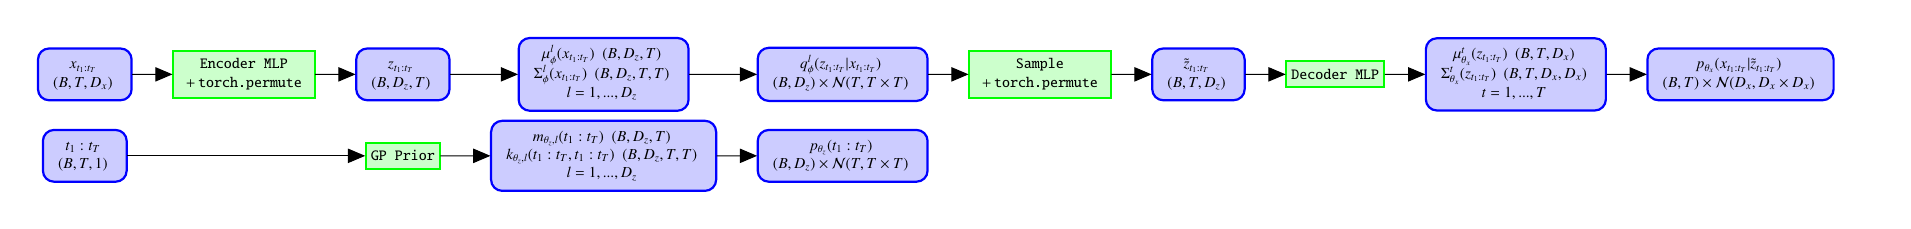
\begin{tikzpicture}[
    % format
    scale=0.55,
    every node/.style={scale=0.55},
    torch/.style={
        rectangle, 
        minimum size=6mm, 
        thick, 
        draw=green!100, 
        fill=green!20, 
        font=\ttfamily
        },
    math/.style={
        rectangle, 
        rounded corners, 
        thick, 
        draw=blue!100,
        fill=blue!20,
        align=center,
        anchor=center,
        inner sep=5pt
        },
    point/.style={
        circle,
        inner sep=0pt,
        minimum size=0pt,
        }
    ]
    % place nodes
    \matrix[row sep = 1mm, column sep=5mm] {
    % row 1
        \node[math] (xt) {
        $\begin{array}{c}
                x_{t_1:t_T} \\
                (B,T,D_x)
        \end{array}$
        }; & 
        \node[torch] (encoder) {
        $\begin{array}{c}
            \text{\ttfamily{Encoder MLP}} \\
            + \, \text{\ttfamily{torch.permute}}
        \end{array}$
        }; &
        \node[math] (zt_perm) {
        $\begin{array}{c}
                z_{t_1:t_T} \\
                (B,D_z,T)
        \end{array}$
        }; & 
        \node[math] (phi) {
            $\begin{array}{c}
                    \mu_{\phi}^l(x_{t_1:t_T}) \,\,\, (B,D_z,T)\\
                    \Sigma_{\phi}^l(x_{t_1:t_T}) \,\,\, (B,D_z,T,T) \\
                    l=1,...,D_z
            \end{array}$
        }; & 
        \node[math] (q_phi) {
        $\begin{array}{c}
        q_{\phi}^l(z_{t_1:t_T} \vert x_{t_1:t_T} ) \\
        (B,D_z) \times \mathcal{N}(T, T\times T)
        \end{array}$
        }; &
        \node[torch] (sample) {
        $\begin{array}{c}
        \text{\ttfamily{Sample}} \\
        + \, \text{\ttfamily{torch.permute}}
        \end{array}$
        }; &
        \node[math] (zt_tilde_perm) {
        $\begin{array}{c}
                \tilde{z}_{t_1:t_T} \\
                (B,T,D_z)
        \end{array}$
        }; & 
        \node[torch] (decoder) {Decoder MLP}; &
        \node[math] (theta_x) {
            $\begin{array}{c}
                    \mu_{\theta_x}^t(z_{t_1:t_T}) \,\,\, (B,T,D_x)\\
                    \Sigma_{\theta_x}^t(z_{t_1:t_T}) \,\,\, (B,T,D_x,D_x) \\
                    t=1,...,T
            \end{array}$
        }; & 
        \node[math] (p_theta_x) {
        $\begin{array}{c}
        p_{\theta_x}(x_{t_1:t_T} \vert \tilde{z}_{t_1:t_T} ) \\ 
        (B,T) \times \mathcal{N}(D_x, D_x\times D_x) \\
        \end{array}$
        }; & \\
    % row 2
    \node[math] (times) {
        $\begin{array}{c}
                {t_1:t_T} \\
                (B,T,1)
        \end{array}$
        }; & &  
    \node[torch] (prior) {GP Prior}; &
    \node[math] (theta_z) {
            $\begin{array}{c}
                    m_{\theta_z, l}({t_1:t_T}) \,\,\, (B,D_z,T)\\
                    k_{\theta_z, l}({t_1:t_T,t_1:t_T}) \,\,\, (B,D_z,T,T) \\
                    l=1,...,D_z
            \end{array}$
        }; &  
    \node[math] (p_theta_z) {
        $\begin{array}{c}
        p_{\theta_z}({t_1:t_T}) \\ 
        (B,D_z) \times \mathcal{N}(T, T\times T) \\
        \end{array}$
        }; & \\
    };
    % draw edges
    \path   (xt) edge [->, thin] (encoder)
            (encoder) edge [->, thin] (zt_perm)
            (zt_perm) edge [->, thin] (phi)
            (phi) edge [->, thin] (q_phi)
            (q_phi) edge [->, thin] (sample)
            (sample) edge [->, thin] (zt_tilde_perm)
            (zt_tilde_perm) edge [->, thin] (decoder)
            (decoder) edge [->, thin] (theta_x)
            (theta_x) edge [->, thin] (p_theta_x)
            (times) edge[->, thin] (prior)
            (prior) edge[->, thin] (theta_z)
            (theta_z) edge[->, thin] (p_theta_z);
\end{tikzpicture}

% --- Loss GPVAE
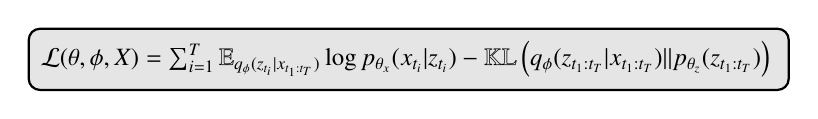
\begin{tikzpicture}[
    scale=0.90,
    every node/.style={scale=0.90},
    math/.style={
        rectangle, 
        % minimum height=1cm,
        % minimum width=2cm,
        rounded corners, 
        thick, 
        draw=black!100,
        fill=gray!20,
        align=center,
        anchor=center,
        inner sep=5pt
        },
    ]
    \node[math] {
        $\VLB = \sum_{i=1}^T \E{q_{\phi}(z_{t_i} \vert x_{t_1:t_T})} \log{p_{\theta_x}(x_{t_i} \vert z_{t_i})} - \KL{q_{\phi}(z_{t_1:t_T} \vert x_{t_1:t_T})}{p_{\theta_z}(z_{t_1:t_T})}$
    };
\end{tikzpicture}

\caption{Gaussian Process VAE Model Architecture}
\end{centering}
\end{figure}

\end{landscape}

         
    % \chapter{Torch implementation take-aways}\label{sec:Torch implementation}

%
%
%------- DEEP KALMAN FILTER ------------------------------
%
%

\begin{landscape}
\begin{figure}
\begin{centering}
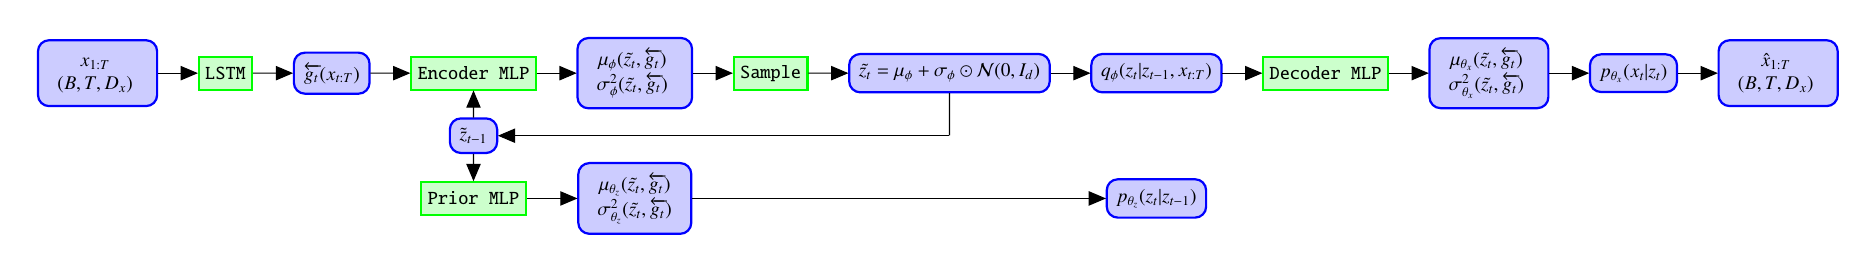
\begin{tikzpicture}[
    scale=0.70,
    every node/.style={scale=0.70},
    torch/.style={
        rectangle, 
        minimum size=6mm, 
        thick, 
        draw=green!100, 
        fill=green!20, 
        font=\ttfamily
        },
    math/.style={
        rectangle, 
        % minimum height=1cm,
        % minimum width=2cm,
        rounded corners, 
        thick, 
        draw=blue!100,
        fill=blue!20,
        align=center,
        anchor=center,
        inner sep=5pt
        },
    point/.style={
        circle,
        inner sep=0pt,
        minimum size=0pt,
        }
    ]
\matrix[row sep = 1mm, column sep=5mm] {
% first row
\node[math] (xt) {
    $\begin{array}{c}
            x_{1:T} \\
            (B,T,D_x)
    \end{array}$
}; & 
\node[torch] (lstm) {LSTM}; & 
\node[math] (gt) {$\overleftarrow{g_t}(x_{t:T})$}; &
\node[torch] (enco) {Encoder MLP}; &
\node[math] (phi) {
    $\begin{array}{c}
            \mu_{\phi}(\tilde{z_t}, \overleftarrow{g_t}) \\
            \sigma_{\phi}^2(\tilde{z_t}, \overleftarrow{g_t})
    \end{array}$
}; &
\node[torch] (sample) {Sample}; &
\node[math] (z_tilde) {$\tilde{z_t} = \mu_{\phi} + \sigma_{\phi} \odot \mathcal{N}(0, I_d)$}; &
\node[math] (q_phi) {$q_{\phi}(z_t \vert z_{t-1}, x_{t:T})$}; &
\node[torch] (deco) {Decoder MLP}; &
\node[math] (theta_x) {
    $\begin{array}{c}
        \mu_{\theta_x}(\tilde{z_t}, \overleftarrow{g_t}) \\
        \sigma_{\theta_x}^2(\tilde{z_t}, \overleftarrow{g_t})
    \end{array}$
}; &
\node[math] (p_theta_x) {$p_{\theta_x}(x_t \vert z_t)$}; &
\node[math] (x_hat) {
    $\begin{array}{c}
            \hat{x}_{1:T} \\
            (B,T,D_x)
    \end{array}$
}; \\
%second row
& & & \node[math] (z_t_1) (z_t_1) {$\tilde{z}_{t-1}$}; & & & \node[point] (coin) {}; & & &; \\
%third row
& & & \node[torch] (prior) {Prior MLP}; &
\node[math] (theta_z) {
    $\begin{array}{c}
            \mu_{\theta_z}(\tilde{z_t}, \overleftarrow{g_t}) \\
            \sigma_{\theta_z}^2(\tilde{z_t}, \overleftarrow{g_t})
    \end{array}$}; & & &
\node[math] (p_theta_z) {$p_{\theta_z}(z_t \vert z_{t-1})$}; &
& & \\
};
\path   (xt) edge [->, thin] (lstm)
        (lstm) edge [->, thin] (gt)
        (gt) edge [->, thin] (enco)
        (enco) edge [->, thin] (phi)
        (phi) edge [->, thin] (sample)
        (sample) edge [->, thin] (z_tilde)
        (z_tilde) edge [->, thin] (q_phi)
        (q_phi) edge[->, thin] (deco)
        (deco) edge [->, thin] (theta_x)
        (theta_x) edge [->, thin] (p_theta_x)
        (p_theta_x) edge [->, thin] (x_hat)
        (z_t_1) edge [->, thin] (enco)
        (prior) edge [<-, thin] (z_t_1)
        (theta_z) edge [<-, thin] (prior)
        (theta_z) edge[->, thin] (p_theta_z)
        (z_tilde) edge [-, thin] (coin)
        (coin) edge [->, thin] (z_t_1);
\end{tikzpicture}

% --- Loss DKF
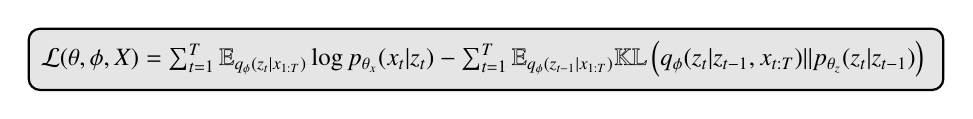
\begin{tikzpicture}[
    scale=0.90,
    every node/.style={scale=0.90},
    math/.style={
        rectangle, 
        % minimum height=1cm,
        % minimum width=2cm,
        rounded corners, 
        thick, 
        draw=black!100,
        fill=gray!20,
        align=center,
        anchor=center,
        inner sep=5pt
        },
    ]
    \node[math] {
            $\VLB = \sum_{t=1}^T \E{q_\phi(z_{t} \vert x_{1:T})} \log{p_{\theta_x}(x_t \vert z_t)} - \sum_{t=1}^T \E{q_\phi(z_{t-1} \vert x_{1:T})} \KL{q_{\phi}(z_t \vert z_{t-1}, x_{t:T})}{p_{\theta_z}(z_t \vert z_{t-1})}$
    };
\end{tikzpicture}

\end{centering}
\caption{Deep Kalman Filter Model Architecture}
\end{figure}
% \end{landscape}


%
%
% ----- VARIATIONAL RNN ------------------
%
%

% \begin{landscape}
\begin{figure}
\begin{centering}
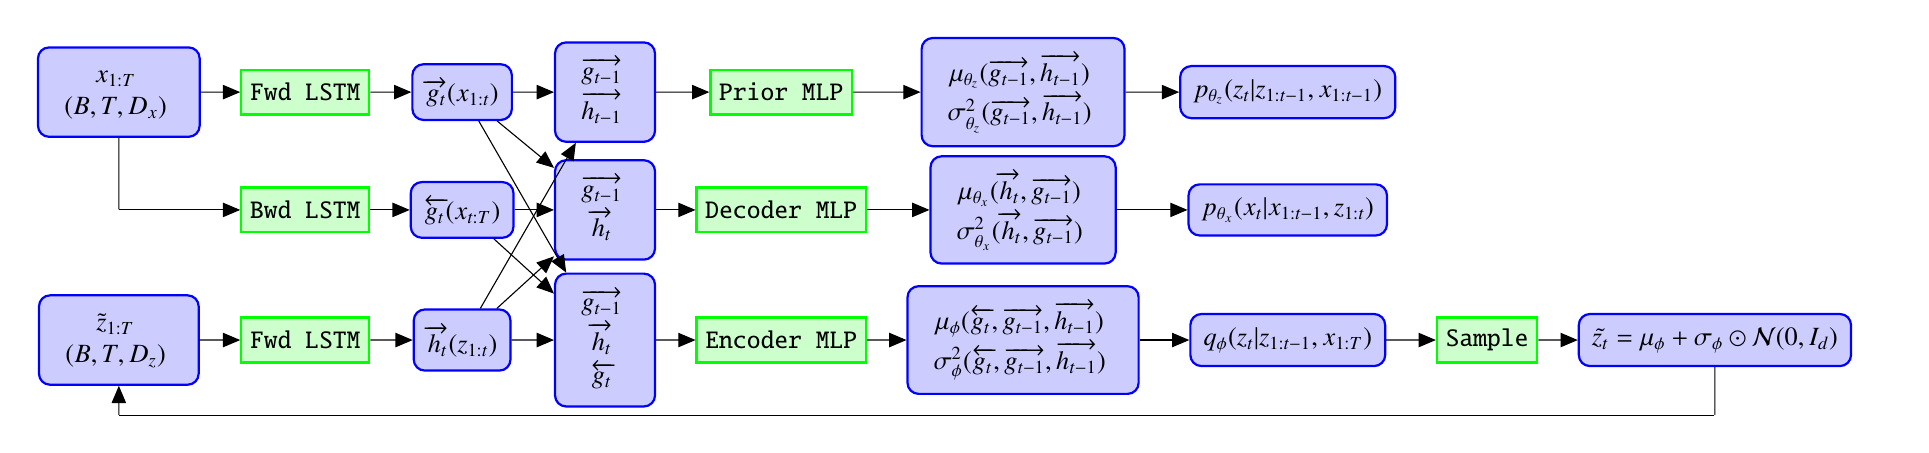
\begin{tikzpicture}[
    % format
    scale=0.95,
    every node/.style={scale=0.95},
    torch/.style={
        rectangle, 
        minimum size=6mm, 
        thick, 
        draw=green!100, 
        fill=green!20, 
        font=\ttfamily
        },
    math/.style={
        rectangle, 
        rounded corners, 
        thick, 
        draw=blue!100,
        fill=blue!20,
        align=center,
        anchor=center,
        inner sep=5pt
        },
    point/.style={
        circle,
        inner sep=0pt,
        minimum size=0pt,
        }
    ]
\matrix[row sep = 1mm, column sep=5mm] {
% row 1
\node[math] (xt) {
    $\begin{array}{c}
            x_{1:T} \\
            (B,T,D_x)
    \end{array}$
}; & 
\node[torch] (fwd_lstm) {Fwd LSTM}; & 
\node[math] (gt) {$\overrightarrow{g_t}(x_{1:t})$}; &
\node[math] (g_t_1_et_h_t_1) {
    $\begin{array}{c}
        \overrightarrow{g_{t-1}} \\
        \overrightarrow{h_{t-1}}
    \end{array}$
}; &
\node[torch] (prior) {Prior MLP}; &
\node[math] (theta_z) {
    $\begin{array}{c}
            \mu_{\theta_z}(\overrightarrow{g_{t-1}}, \overrightarrow{h_{t-1}}) \\
            \sigma_{\theta_z}^2(\overrightarrow{g_{t-1}}, \overrightarrow{h_{t-1}})
    \end{array}$
}; &
\node[math] (p_theta_z) {$p_{\theta_z}(z_t \vert z_{1:t-1}, x_{1:t-1})$}; & \\
% row 2
\node[point] (coin3) {}; &
\node[torch] (bwd_lstm) {Bwd LSTM}; & 
\node[math] (gt2) {$\overleftarrow{g_t}(x_{t:T})$}; &
\node[math] (g_t_1_et_h_t) {
    $\begin{array}{c}
        \overrightarrow{g_{t-1}} \\
        \overrightarrow{h_{t}}
    \end{array}$
}; &
\node[torch] (decoder) {Decoder MLP}; &
\node[math] (theta_x) {
    $\begin{array}{c}
            \mu_{\theta_x}(\overrightarrow{h_t}, \overrightarrow{g_{t-1}}) \\
            \sigma_{\theta_x}^2(\overrightarrow{h_t}, \overrightarrow{g_{t-1}})
    \end{array}$
}; & 
\node[math] (p_theta_x) {$p_{\theta_x}(x_t \vert x_{1:t-1}, z_{1:t} )$}; & \\
% row 3
\node[math] (z_tilde) {
    $\begin{array}{c}
            \tilde{z}_{1:T} \\
            (B,T,D_z)
    \end{array}$
}; & 
\node[torch] (fwd_lstm2) {Fwd LSTM}; & 
\node[math] (ht) {$\overrightarrow{h_t}(z_{1:t})$}; &
\node[math] (g_t_1_et_h_t_1_et_g_t) {
    $\begin{array}{c}
        \overrightarrow{g_{t-1}} \\
        \overrightarrow{h_{t}} \\
        \overleftarrow{g_t}
    \end{array}$
}; &
\node[torch] (encoder) {Encoder MLP}; &
\node[math] (phi) {
    $\begin{array}{c}
            \mu_{\phi}(\overleftarrow{g_{t}}, \overrightarrow{g_{t-1}}, \overrightarrow{h_{t-1}}) \\
            \sigma_{\phi}^2(\overleftarrow{g_{t}}, \overrightarrow{g_{t-1}}, \overrightarrow{h_{t-1}})
    \end{array}$
}; & 
\node[math] (q_phi) {$q_{\phi}(z_t \vert z_{1:t-1}, x_{1:T} )$}; &
\node[torch] (sample) {Sample}; &
\node[math] (z_tilde_formula) {$\tilde{z_t} = \mu_{\phi} + \sigma_{\phi} \odot \mathcal{N}(0, I_d)$}; & \\
% row 4
\node[point] (coin1) {};
& & & & & & & &;
\node[point] (coin2) {}; & \\
};
\path   (xt) edge [->, thin] (fwd_lstm)
        (xt) edge[-, thin] (coin3)
        (fwd_lstm) edge [->, thin] (gt)
        (gt) edge[->, thin] (g_t_1_et_h_t_1)
        (gt) edge[->, thin] (g_t_1_et_h_t)
        (gt) edge[->, thin] (g_t_1_et_h_t_1_et_g_t)
        (g_t_1_et_h_t_1) edge[->, thin] (prior)
        (prior) edge[->, thin] (theta_z)
        (theta_z) edge[->, thin] (p_theta_z)
        (coin3) edge[->, thin] (bwd_lstm)
        (bwd_lstm) edge[->, thin] (gt2)
        (gt2) edge[->, thin] (g_t_1_et_h_t)
        (gt2) edge[->, thin] (g_t_1_et_h_t_1_et_g_t)
        (g_t_1_et_h_t) edge[->, thin] (decoder)
        (decoder) edge[->, thin] (theta_x)
        (theta_x) edge[->, thin] (p_theta_x)
        (z_tilde) edge[->, thin] (fwd_lstm2)
        (fwd_lstm2) edge[->, thin] (ht)
        (ht) edge[->, thin] (g_t_1_et_h_t_1_et_g_t)
        (ht) edge[->, thin] (g_t_1_et_h_t)
        (ht) edge[->, thin] (g_t_1_et_h_t_1)
        (g_t_1_et_h_t_1_et_g_t) edge[->, thin] (encoder)
        (encoder) edge[->, thin] (phi)
        (phi) edge[->, thin] (q_phi)
        (q_phi) edge[->, thin] (sample)
        (sample) edge[->, thin] (z_tilde_formula)
        (z_tilde_formula) edge[-, thin] (coin2)
        (coin2) edge[-, thin] (coin1)
        (coin1) edge[->, thin] (z_tilde);
\end{tikzpicture}

% --- Loss VRNN
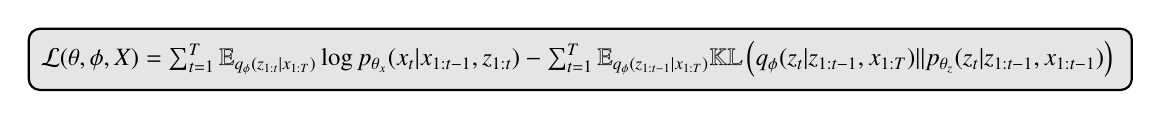
\begin{tikzpicture}[
    scale=0.90,
    every node/.style={scale=0.90},
    math/.style={
        rectangle, 
        % minimum height=1cm,
        % minimum width=2cm,
        rounded corners, 
        thick, 
        draw=black!100,
        fill=gray!20,
        align=center,
        anchor=center,
        inner sep=5pt
        },
    ]
    \node[math] {
        $\VLB = \sum_{t=1}^T  \E{q_{\phi}(z_{1:t} \vert x_{1:T})} \log{p_{\theta_x}(x_t \vert x_{1:t-1}, z_{1:t})} - \sum_{t=1}^T \E{q_{\phi}(z_{1:t-1} \vert x_{1:T})} \KL{q_{\phi}(z_t \vert z_{1:t-1}, x_{1:T})}{p_{\theta_z}(z_t \vert z_{1:t-1}, x_{1:t-1})}$
    };
\end{tikzpicture}

\end{centering}
\caption{Variational RNN Model Architecture}
\end{figure}

\end{landscape}

    % \include{chapter/Torch_implementation_take_aways_2}

% 
%
% ------- STOCHASTIC CALCULUS BASICS, SDE AND DVAE ---------------------------
%
%

\part{Notions on stochastic differential equations and their relationships to DVAEs}

This part intends to present a self-contained "survival kit" material on stochastic calculus, in order to highlight the relationships between \glspl{sde} and \glspl{dvae}.

NB : stochastic calculus is a full mathematical field in itself, and a more detailed presentation is located at the very end of this report. For a full study
of the matter, the interested reader will likely enjoy \cite{mouvement-brownien-calcul-ito}, \cite{sarkka_applied_2019}, and refer to \cite{cours-jf-legall}.

    \include{chapter/Entropy_and_randomness}
    \chapter{Stochastic calculus intoduction}\label{sec:SC_intro}

This chapter is a reminder of some key notions of stochastic calculus. 
More details are presented at the end of the report, and in \cite{mouvement-brownien-calcul-ito}, \cite{sarkka_applied_2019}.

A \textbf{stochastic process} is formally defined as:

\defn{Stochastic process}{
    A stochastic process $X$ is defined as:
\begin{align}
    X &= (\Omega, \mathcal{F}, (X_t)_{t \in T}, \mathbb{P}) \\
    &= (\Omega, \mathcal{F}, (\mathcal{F}_t)_{t \in T}, (X_t)_{t \in T}, \mathbb{P})
\end{align}
where:
    \begin{itemize}
        \item $\Omega$ is a set (universe of possibles).
        \item $\mathcal{F}$ is a $\sigma$-algebra of parts of $\Omega$
        \item $\mathbb{P}$ is a probability measure on $(\Omega, \mathcal{F})$
        \item $T \subset \mathbb{R}_+$ represents time
        \item $(\mathcal{F}_t)_{t \in T}$ is a \textbf{filtration}, ie an increasing family of sub-$\sigma$-algebras of $\mathcal{F}$ indexed by $t$ : $\forall 0 \leq s \leq t \in T$, $\mathcal{F}_s \subset \mathcal{F}_t \subset \mathcal{F}$.
        \item $(X_t)_{t \in T}$ is a family of RV defined on $(\Omega, \mathcal{F})$ with values in a measurable space $(E, \mathcal{E})$ or more simply $(E, \mathcal{B}(E))$ (set $E$ endowed with its Borelian $\sigma$-algebra).
        \item $(X_t)_{t \in T}$ is assumed \textbf{adapted to the filtration} $(\mathcal{F}_t)_{t \in T}$, meaning $\forall t \in T$, $X_t$ is $\mathcal{F}_t$-measurable
    \end{itemize}
}

A filtration $\mathcal{F}_{t\geq 0}$ is often viewed and introduced as the \textit{set of information available at time $t$}. 

The core of stochastic calculus is the stochastic process known as \textbf{Brownian motion}, or \textbf{Wiener process}. 
We use here the definition of a multivariate Brownian motion:

\defn{Brownian motion}{
A stochastic process $B = \brownian$ with values in $\mathbb{R}^d$ is called \textbf{Brownian motion} iff:
\begin{itemize}
    \item $B_0 = 0$ $\mathbb{P}$-a.s.
    \item $\forall 0 \leq s \leq t$, the random variable $B_t-B_s$ is independent from $\mathcal{F}_t$.
    \item $\forall 0 \leq s \leq t$, $B_t - B_s \sim \mathcal{N}(0,Q(t-s))$
    \item $B$ is continuous \footnote{or more exactly there exists a continuous version of $B$, see \cite{mouvement-brownien-calcul-ito}}
\end{itemize}
where the matrix $Q \in \mathbb{S}^{++}_d$ is called the \textbf{diffusion matrix}.
}

Meaning : the process $B$ starts from 0, its increments are independent from the past, its increments over disjoint time intervals are independent of each other, 
its increments follow a centered normal law of variance equal to the length of the time interval multiplied by the diffusion matrix.
NB : some authors choose the define the diffusion matrix (or scalar) outside of the Brownian motion.

A core result is that the quadratic variation of the Brownian motion over an interval $[s,t]$ (equiped
with a subdivison $\pi = \{s=t_0 < t_1 < ...< t_k <... < t_n=t\}$), and defined as the limit when $\vert \pi \vert \rightarrow 0$ 
of $V_{\pi}^{(2)} = \sum_{k=0}^{n-1} \vert f(t_{k+1})-f(t_k)\vert^{2}$, is:

\begin{align}
    &\underset{\vert \pi \vert \rightarrow 0}{\text{lim}}\,\, V_{\pi}^{(2)} = Q(t-s) \,\, \text{in} \,\, L^{2}
\end{align}

Or, heuristically, 
\begin{align}
    \label{dB_square_is_dt}
    \mathbb{E}(dB_t dB_t^T) = Q dt
\end{align}

Ito then proceeds to define \textbf{stochastic integrals}, starting with elementary processes:

\defn{Elementary process}{
A stochastic process $X = (X_s)_{s \in [a,b]}$ is called \textbf{elementary} if there exists a subdivision $a = t_0 < t_1 < ... < t_n = b$ of $[a,b]$, such that:
\[
\forall t \in [a,b], \forall \omega \in \Omega, X_t(\omega) = \sum_{i=0}^{n-1} X_i(\omega) \textbf{1}_{[t_i, t_{i+1}[}(t)
\]
with $\forall i \in \{0,1,..,n-1\}, X_i$ is $\mathcal{F}_{t_i}$-measurable.

This means that, in each interval $[t_i, t_{i+1}[$, $X_t(\omega)$ is independent of $t$ and $X_t(\omega) = X_i(\omega)$.

We define $\mathcal{E}$ (resp. $\mathcal{E}_n, n>0$) the set of all elementary processes on $[a,b]$ (resp. the subset of the $X \in \mathcal{E}$)) such that all $X_i$ have a finite moment $\mathbb{E}X_i <\infty$ (resp $\mathbb{E}(\vert X_i\vert^n) < \infty$
}

\defn{Stochastic integral of an elementary process}{
Let $X \in \mathcal{E}$, ie
\[
X_t(\omega) = \sum_{i=0}^{n-1} X_i(\omega) \textbf{1}_{[t_i, t_{i+1}[}(t)
\]
\textbf{The stochastic integral of $X$ is the real random variable} :
\[
\int_a^b X_t dB_t := \sum_{i=0}^{n-1} X_i (B_{t_{i+1}} - B_{t_{i}})
\]
}

The notion is then extended to other stochastic processes (in spaces of square integrable processes, see the annex).

The definition of a \gls{sde} is derived from the notion of stochastic integral:

\defn{Ito's process}{
    A process $X = (X_t)_{t \in [0, T]}$ is called a \textbf{Ito's process} if it can be written as:
    \begin{align}
        \label{ito sde definition}
        X_t &= X_0 + \int_{0}^{t}a_s ds + \int_{0}^{t} b_s dB_s \,\,\, \forall t \in [0,T]
    \end{align}
    where $a$ and $b$ are two stochastic processes such that the integrals exist (ie $a \in  \Lambda^1$ and 
    $b \in \Lambda^2$).\\
    Equivalently, we write $X_t$ as the soltuion to the \textbf{Stochastic Differential Equation}:
    \begin{align*}
        dX_t = a_t dt + b_t dB_t
    \end{align*}
}

The very famous \textbf{Ito's formula} will allow to make calulations on stochastic processes:

\thmp{Itô's formula}{
An Itô's process remains an Itô's process when it is transformed by a deterministic function that is "smooth enough".

Let $X$ be a Itô's process on $[0,T]$ : $dX_t = a_tdt + b_t dB_t$.

Let:
\begin{align*}
    f : \mathbb{R} \times \mathbb{R} &\rightarrow \mathbb{R} \\
    (x,t) &\mapsto f(x,t)
\end{align*}
be $\mathcal{C}^{2,1}$ : $\mathcal{C}^2$ in $x$, and $\mathcal{C}^1$ in $t$.

Then $(f(X_t,t))_{t \in [0,T]}$ is also an Itô's process and:
\begin{align}
    d\left( f(X_t,t) \right) = \frac{\partial f}{\partial t}(X_t,t) dt + \frac{\partial f}{\partial x}(X_t,t) dX_t + \frac{1}{2}\frac{\partial^2 f}{\partial x^2}(X_t,t)b_t^2 dt
\end{align}
The last term is Itô's complementary term.\\
In dimension $d > 1$:
\begin{align}
    d\left( f(X_t,t) \right) = \frac{\partial f}{\partial t}(X_t,t) dt + ()\nabla f)^T (X_t,t) dX_t + \frac{1}{2}\text{Tr} \left( (\nabla \nabla^T f) dX_t dX_t^T \right)
\end{align}
}{see book \cite{mouvement-brownien-calcul-ito} for a clean proof. A heuristic process can be derived by using a Taylor-Lagrange decomposition at order 2, and using \ref{dB_square_is_dt}}
    \chapter{Stochastic Differential Equations}\label{sec:SDE_results}

\lipsum[1-3]
    % add chapter for links between SDEs and DVAEs
    \chapter{Filtering, Smoothing, and the GP-VAE}\label{sec:filter smoother gps}

Equiped with the stochastic calculus basics, we see in this chapter that the filtering and smoothing 
tasks (ie computing posterior probabilities of the latent variables) provides a complete framework 
for the corresponding tasks in \glspl{dvae}.

We also see that, when a Gaussian process can be formulated as the solution of a linear \gls{sde} (ie
 when the kernel function verifies some properties), then the gaussian process regression problem 
 of computing posterior probabilities can be performed by algorithms in linear time.

In this chapter, we consider \glspl{ct-ssm} and \glspl{cd-ssm}. In both cases, the latent variables are 
defined by a (continuous) \gls{sde}. The observations can be defined by a second \gls{sde}, or by a set of 
discrete-time observations.

Formally, the \gls{ct-ssm} is defined by:

\begin{tcolorbox}[colback=blue!5!white,colframe=black!75!black,title=Continuous-Time State Space model]
    \begin{align}
        dZ_t &= F(Z_t, t)dt + L(Z_t,t) dB_t \\
        dX_t &= H(Z_t,t)dt + d\eta_t
    \end{align}
    where:
    \begin{itemize}
        \item $Z_t \in \mathbb{R}^{D}$ is the \textit{state}, ie a stochastic process defining the latent variable.
        \item $B_t \in \mathbb{R}^{S}$ is a Brownian motion with diffusion matrix $Q$.
        \item $F \in \mathbb{R}^{D}$ and $L \in \mathbb{R}^{D \times S}$ are the usual drift and dispersion functions.
        \item $X_t \in \mathbb{R}^{M}$ is the \textit{integrated} measurement (or observation) process.
        \item $H \in \mathbb{R}^{M}$ is the observation/measurement model.
        \item $\eta_t \in \mathbb{R}^{S}$ is a Brownian motion with diffusion matrix $R$.
    \end{itemize}
    NB : the observations are assumed to conditionnally independent of the state, and $B_t, \eta_t$ are 
     assumed independent.
    The observation model is equivalent to:
    \begin{align}
        y_t &= \frac{dX_t}{dt} = H(Z_t,t) + \epsilon_t \\
        \epsilon_t &= \frac{d \eta_t}{dt}
    \end{align}
\end{tcolorbox}

Formally, the \gls{cd-ssm} is defined by:

\begin{tcolorbox}[colback=blue!5!white,colframe=black!75!black,title=Continuous-Discrete State Space model]
    \begin{align}
        dZ_t &= F(Z_t, t)dt + L(Z_t,t) dB_t \\
        x_k &\sim p(x_k \vert z_{t_k})
    \end{align}
    where:
    \begin{itemize}
        \item $Z_t \in \mathbb{R}^{D}$ is the \textit{state}, ie a stochastic process defining the latent variable.
        \item $B_t \in \mathbb{R}^{S}$ is a Brownian motion with diffusion matrix $Q$.
        \item $F \in \mathbb{R}^{D}$ and $L \in \mathbb{R}^{D \times S}$ are the usual drift and dispersion functions.
        \item $x_k$ are the observations taken at \textbf{discrete times $(t_k)_{k=1,...,n}$}
    \end{itemize}
    NB : the observations are assumed to conditionnally independent of the state.
\end{tcolorbox}

We see that the \gls{gpvae} is a specific \gls{cd-ssm}, where the underlying latent stochastic process 
is actually a Gaussian process.

Also, the \gls{ct-ssm} assumes a Gaussian observation model, whereas the \gls{cd-ssm} allows more general 
observation models.

From a vocabulary stand-point, we will use indifferently \textit{state} or \textit{latent variable}, and 
\textit{observation} or \textit{measurement}.

\section{Filtering and Smooting}

\textbf{Filtering} is the problem of determining the posterior probability of the latent $Z_t$ given the 
discrete measurements \textbf{up to $t$}, ie finding $p(Z_t \vert x_{1:k})$ with $t_k \leq t$. This corresponds to 
determining the generative transition probability $p_{\theta_z}(z_t \vert z_{1:t-1}, x_{1:t-1})$ in our 
\gls{dvae} setting.

In general, close-form solutions can be derived when the latent variables \gls{sde} is linear. In continuous 
time, we get the \textbf{Kalman-Bucy} filter equations, which discretize in the well-known \textbf{Kalman filter}.

\begin{tcolorbox}[colback=blue!5!white,colframe=black!75!black,title=Kalman-Bucy filter]
    \begin{align}
        dZ_t &= F(t)Z_t dt + L(t) dB_t \\
        dX_t &= H(t)X_t dt + d\eta_t
    \end{align}
    where:
    \begin{itemize}
        \item $Z_t \in \mathbb{R}^{D}$ is the state/latent.
        \item $X_t \in \mathbb{R}^{M}$ is the observation/measurement.
        \item $B_t \in \mathbb{R}^{S}$ is a Brownian motion with diffusion matrix $Q$.
        \item $\eta_t \in \mathbb{R}^{S}$ is a Brownian motion with diffusion matrix $R$.
        \item $F \in \mathbb{R}^{D}$ and $L \in \mathbb{R}^{D \times S}$ are the usual drift/dynamic model and dispersion functions.
        \item $H \in \mathbb{R}^{D \times M}$ is the measurement/observation model
    \end{itemize}
    NB : the observations are assumed to conditionnally independent of the state.
    Then the Bayesian filter (Kalman-Bucy) is:
    \begin{align}
        p(z_t \vert x_{<t}) &= \mathcal{N}(Z_t \vert m_t, P_t) \\
        K &= P H(t)^{T} R^{-1} \\
        dm &= F(t)m dt + K (dX_t - H(t) m dt) \\
        \frac{dP}{dt} &= F(t)P + P F(t)^{T} + L(t)QL(t)^{T} - KRK^{T}
    \end{align}
\end{tcolorbox}

In practice, one can approximate a general \gls{sde} by a linear \gls{sde} and apply Kalman-Bucy.

\textbf{Smoothing} is the problem of determining the posterior probability of the latent $Z_t$ given 
all known observations, ie finding $p(Z_t \vert x_{1:T})$ for all $t \in [0,T]$. This corresponds to 
determining the inference model $q_{\phi}(z_t \vert z_{1:t-1}, x_{1:T})$ in the \gls{dvae} setting.

We describe here briefly the \gls{rts} smoother for discrete time models.

Discretizing the transition density in \gls{cd-ssm}, we have
\begin{align}
    Z_{t_{k+1}} &\sim p(Z_{t_{k+1}} \vert Z_{t_k}) \\
    X_k &\sim p(X_k \vert Z_{t_k})
\end{align}

And the smoothers:

\begin{tcolorbox}[colback=blue!5!white,colframe=black!75!black,title=Bayesian smoother]
    \begin{align}
        Z_{t_{k+1}} &\sim p(Z_{t_{k+1}} \vert Z_{t_k}) \\
        X_k &\sim p(X_k \vert Z_{t_k})
    \end{align}
    The \textit{Bayesian smoother} is, for any $k < T$:
    \begin{align}
        p(Z_{t_{k+1}} \vert X_{1:k}) &= \int p(Z_{t_{k+1}} \vert Z_{t_k}) p(Z_{t_k} \vert X_{1:k}) dZ_{t_k} \\
        p(Z_{t_k} \vert X_{1:T}) &= p(Z_{t_{k}} \vert X_{1:k})\int \left(
            \frac{
                p(Z_{t_{k+1}} \vert Z_{t_k}) p(Z_{t_{k+1}} \vert X_{1:T})
            }{
                p(Z_{t_{k+1}} \vert X_{1:k}
            }dZ_{t_{k+1}}
        \right)
    \end{align}
    The backward recursion is started from the final step, where the filtering and smoothing densities 
    are the same : $p(Z_{t_T} \vert X_{1:T})$.
\end{tcolorbox}

The \gls{rts} smoother is the close-form solution of the Bayesian filter for a linear Gaussian problem 
- see \cite{sarkka_applied_2019} for the algorithm.

\section{GP-VAE}

We wrap up here linking the filtering/smoothing theory of linear \gls{sde} with the \gls{gpvae} 
model of \cite{fortuin_gp-vae:_2020}.

If we use the formalization above, a \gls{gpvae} is basically:

\begin{align}
    \label{gpvae sde form}
    Z_t &\sim \mathcal{GP}(m(\bullet), k(\bullet, \bullet)) \\
    X_{t_k} &\sim p(X_{t_k} \vert Z_{t_k})
\end{align}

If we assume that the observation model is Gaussian, then we get
\begin{align}
    \label{gpvae gaussian observation}
    Z_t &\sim \mathcal{GP}(m(\bullet), k(\bullet, \bullet)) \\
    X_{t_k} &\sim \mathcal{N}(X_{t_k} \vert Z_{t_k}, \sigma^{2})
\end{align}

Computing the posterior distribution $p(Z_t \vert X_{t_1:t_T})$ is performing a Gaussian Process 
regression (see \cite{rasmussen_gaussian_2008}), which naively scales in $O(n^{3})$.

However, if the Gaussian process can be written as a linear \gls{sde}:
\begin{align}
    \label{gpvae linear sde form}
    dZ_t &= F(t)Z_t dt + L(t)dB_t \\
    X_{t_k} &\sim \mathcal{N}(X_{t_k} \vert Z_{t_k}, \sigma^{2})
\end{align}

then the Kalman filter and smoother apply, that scale in $O(n)$. This is the main idea in \cite{zhu_markovian_2023}.

However - the solutions of linear \gls{sde} are Gaussian Processes, but the converse is not true. 
More specifically, some kernel functions are such that the associated \gls{gp} can not be represented as 
the solution of a linear \gls{sde}.

For a given kernel function $k(t,t')$, \cite{sarkka_applied_2019} aims at finding a linear time-invariant model
\begin{align}
    dZ_t &= F Z_t dt + L dB_t \\
    X_{t_k} &\sim \mathcal{N} (X_{t_k} \vert H Z_{t_k} , \sigma^{2})
\end{align}
with $Z_t \in  \mathbb{R}^{D}$, but $X_t \in \mathbb{R}$ is one-dimensional (ie $H \in \mathbb{R}^{1 \times D}$), 
and such that $z_t = H Z_t$ is a Gaussian process with kernel $k$.

We give now some examples, and counter-examples, of such associations.

\begin{itemize}
    \item \textbf{Brownian motion} : the Brownian motion is the solution of $dZ_t = dB_t$, 
    and a \gls{gp} with kernel $k(t,t') = \text{min}(t,t')$ (see \ref{sec:brownian_motion_gaussian_and_markov})
    \item \textbf{Ornstein Uhlenbeck} : the O.U. process
    \begin{align}
        dZ_t &= - \frac{1}{l} Z_t dt + dB_t
    \end{align}
    where $dB_t$ has diffusion coefficient $\frac{2 \sigma^{2}}{l}$, is a \gls{gp} with kernel:
    \begin{align}
        k_{\text{exp}} &= \sigma^{2} \exp{(- \frac{\vert t-t' \vert}{l})}
    \end{align}
    \item \textbf{Matern} : the \gls{sde} representation with
    \begin{align}
        F &= \begin{pmatrix}
            0 & 1 \\
            -\lambda^{2} & -2 \lambda 
        \end{pmatrix} \\
        L &= \begin{pmatrix}
            0 \\ 1
        \end{pmatrix} \\
        H &= \begin{pmatrix}
            1 \\ 0
        \end{pmatrix}
    \end{align}
    is a \gls{gp} with the Matern kernel with $\nu = \frac{3}{2}$:
    \begin{align}
        k_{\text{Matern}} &= \sigma^{2} \left(
            1 + \frac{\sqrt{3} \vert t-t' \vert}{l}
        \right) \exp{
            \left(
                -\frac{\sqrt{3} \vert t-t' \vert}{l}
            \right)
        }
    \end{align}
    and $\lambda = \frac{\sqrt{3}}{l}$, diffusion is $q = 4\lambda^{3}\sigma^{2}$.
\end{itemize}

Conversely, the following kernels can not be used to derive an associated linear \gls{sde}:

\begin{itemize}
    \item \textbf{squared exponential} : the widely used
    \begin{align}
        k_{\text{se}}(t,t') &= \sigma^{2} \exp{\left(
            - \frac{\vert t-t' \vert^{2}}{2l^{2}}
        \right)}
    \end{align}
    \item \textbf{rational quadratic}:
    \begin{align}
        k_{\text{rq}}(t,t') &= \sigma^{2} \left(
            1 + \frac{\vert t-t' \vert^{2}}{2 \alpha l^{2}}
        \right)^{-\alpha}
    \end{align}
    with $\alpha > 0$.
\end{itemize}

In that latter case, one can use spectral decomposition (ie Mercer's theorem, see MVA kernel class \cite{mva_kernel_class}) 
to approximate the kernel function and determine an associated linear \gls{sde}.

\part{Experiments}

    \chapter{Experiments}

XPs

Using SPRITES dataset from \cite{li_disentangled_2018}

\part{Conclusion and Discussion}

    \chapter{Conclusions}\label{sec:Conclusions}

\lipsum[1-3]

%
%
% ----- STOCHASTIC CALCULUS IN DETAILS ---------------------
%
%
\part{More on stochastic calculus}

    \chapter{Stochastic processes main theory}\label{sec:Stochastic_Processes}
    
% \section{Definition and properties of a stochastic process}

We posit the following in the rest of the doc, unless specified otherwise:
% \begin{tcolorbox}[colback=blue!5!white,colframe=black!75!black,title=]
\asum{Main assumptions}{
\begin{enumerate}
    \item $(\Omega, \mathcal{F}, \mathbb{P})$ is a probabilistic space, with $\Omega$ the universe, $\mathcal{F}$ the tribe ($\sigma$-algebra) of events, $\mathbb{P}$ a probability measure on $(\Omega,\mathbb{F})$.
    \item $(E, \mathbb{B}(E))$ is a measurable space, endowed with its Borelian $\sigma$-algebra. $E$ will sometimes be referred to as the \textit{state space}. It is typically the space where random variables will live, most of the time $(\mathbb{R}, \mathcal{B}(\mathbb{R})).$
    \item $T$ is the set of \textit{times}, typically $T = [0, a]$ with $a>0$, or $T=[0, +\infty[$.
\end{enumerate}
}

% \subsection{Intuition and definitions }

We view a stochastic process as a two-variable function from $T \times \Omega$ to $(E, \mathcal{B}(E))$:
\begin{align}
    X : T \times \Omega &\longrightarrow (E, \mathcal{B}(E)) \\
    (t, \omega) &\longmapsto X(t, \omega)
\end{align}

This leads to two complementary views:

\textbf{Stochastic process as a collection of random variables indexed by time}
We view $X$ as a collection of random variables $(X_t)_{t \in T}$:
\begin{align}
    \forall t \in T, X_t : \omega \mapsto X_t(\omega)
\end{align}
\begin{enumerate}
    \item Each random variable $X_t$ is defined on $(\Omega, \mathcal{F}, \mathbb{P}$
    \item In practice, only some events $A \in \mathcal{F}$ can occur during the times $[0, t] \in T$. We will note $\mathcal{F}_t$ the smallest $\sigma$-algebra that contains the set of events $A$ that can occur during $[0, t]$.
    \item As a result, $X_t$ must be $\mathcal{F}_t$-measurable.
\end{enumerate}
% }

An alternate view arises when we fix $\omega$ and allow $t \in T$:

\textbf{Stochastic process as a set of random trajectories}
We view $X$ as
\begin{align}
    X : \Omega &\longrightarrow \mathbb{R}^T \\
    \omega &\longmapsto X(\omega) : t \mapsto X(t,\omega)
\end{align}
\begin{enumerate}
    \item $\forall \omega \in \Omega$, $X(\omega) \in \mathbb{R}^T$ is a random trajectory from $T$ into $\mathbb{R}$
    \item $\mathbb{R}^T$ should be endowed with an appropriate $\sigma$-algebra.
\end{enumerate}

Those intuitions lead to a formal definition :

\defn{Stochastic process}{
A stochastic process $\textbf{X}$ is defined as:
\begin{align}
    X &= (\Omega, \mathcal{F}, (X_t)_{t \in T}, \mathbb{P}) \\
    &= (\Omega, \mathcal{F}, (\mathcal{F}_t)_{t \in T}, (X_t)_{t \in T}, \mathbb{P})
\end{align}
where:
    \begin{itemize}
        \item $\Omega$ is a set (universe of possibles).
        \item $\mathcal{F}$ is a $\sigma$-algebra of parts of $\Omega$
        \item $\mathbb{P}$ is a probability measure on $(\Omega, \mathcal{F})$
        \item $T \subset \mathbb{R}_+$ represents time
        \item $(\mathcal{F}_t)_{t \in T}$ is a \textbf{filtration}, ie an increasing family of sub-$\sigma$-algebras of $\mathcal{F}$ indexed by $t$ : $\forall 0 \leq s \leq t \in T$, $\mathcal{F}_s \subset \mathcal{F}_t \subset \mathcal{F}$.
        \item $(X_t)_{t \in T}$ is a family of RV defined on $(\Omega, \mathcal{F})$ with values in a measurable space $(E, \mathcal{E})$ or more simply $(E, \mathcal{B}(E))$ (set $E$ endowed with its Borelian $\sigma$-algebra).
        \item $(X_t)_{t \in T}$ is assumed \textbf{adapted to the filtration} $(\mathcal{F}_t)_{t \in T}$, meaning $\forall t \in T$, $X_t$ is $\mathcal{F}_t$-measurable
    \end{itemize}
}

Often, we will have $(E, \mathcal{B}(E)) = (\mathbb{R}^d, \mathcal{B}(\mathbb{R}^d))$, and $T = [0,a]$ or $T=[0, +\infty[$ or $T=\mathbb{N}$.

Other important notions:
\begin{itemize}
    \item \textbf{$\sigma$-algebra generated by a random variable}. Let $X : (\Omega, \mathcal{F}, \mathbb{P}) \rightarrow (E, \mathcal{E})$ a random variable. The $\sigma$-algebra generated by $X$ is the smallest $\sigma$-algebra that makes $X$-measurable. It is the set of "pre-images" of $\mathcal{B}(E)$ by $X$. Formally;
    \begin{align}
        \sigma(X) = \{ A = X^{-1}(B), B \in \mathcal{E} \}
    \end{align}
    \item \textbf{natural filtration of $(X_t)_{t \in T}$}. The set of $\mathcal{F}_t = \sigma(X_s, s \leq t), \forall t \in T$, ie the set of $\sigma$-algebras generated by the RV $X_s$ for $s \leq t$, is called the natural filtration of $(X_t)$
\end{itemize}

% \subsection{Other definitions and properties}

\defn{Finite dimension laws of a stochastic process}{
Let $X$ be a stochastic process, $I = \{t_1,t_2,...,t_n\}, t_1<t_2<...<t_n$ a finite part of $T$, and $X_I = (X_{t_1}, X_{t_2},...,X_{t_n}) \in E^I$ a random vector.

Then, the \textbf{law of the random vector $X_I$} is the probability measure $\mu_I$ image of $\mathbb{P}$ by $X_I : \Omega \rightarrow (E^I, \mathcal{B}(E^I))$
}

We also remind of Gaussian processes -with a view different from \cite{rasmussen_gaussian_2008}.

% \section{Gaussian vector and gaussian process}

\defn{Gaussian vector}{
Let $\xi = (X_1,X_2,...,X_n)$ be a \textbf{centered} random vector in $\mathbb{R}^n$ ($\mathbb{E}(\xi)=0$), verifying $\xi \in L^2(\Omega, \mathcal{F}, \mathbb{P})$ (ie $\forall i, \mathbb{E}(X_i^2)< \infty$). Let $\Gamma = \mathbb{E}(X_i X_j)\vert_{i,j}$ its covariance matrix (definite positive).

\textbf{$\xi$ is a Gaussian vector} iff, equivalently:
\begin{enumerate}
    \item $\forall a_1,a_2,...,a_n \in \mathbb{R}^n$, $\sum_{i=1}^n a_i X_i$ follows a normal law (ie is Gaussian)
    \item or : the characteristic function of $\xi$, $\Phi_\xi(t)=\mathbb{E}(e^{i<\xi \vert t>})$, can be written
    \begin{align*}
        \Phi_\xi(t)=e^{-\frac{1}{2}<t \vert \Gamma t>} \,\, (t \in \mathbb{R}^n)
    \end{align*}
\end{enumerate}
With notation $\xi \sim \mathcal{N}(0,\Gamma)$.

More generally,
\begin{align*}
    Z \sim \mathcal{N}(m,\Gamma) \iff \Phi_Z(t) = e^{i <m \vert t>} e^{-\frac{1}{2}<t \vert \Gamma t>}
\end{align*}
}

\defn{Gaussian Process}{
Let $X$ be a stochastic process taking its values in $E = \mathbb{R}^n$. 

\textbf{$X$ is said to be a Gaussian process iff all its finite dimension laws are Gaussian}.

If $X = (X_t)_{t\in T}$ is a real-valued Gaussian process ($E=\mathbb{R}$), we define $\forall s,t \in T$:
\begin{itemize}
    \item $m(t)= \mathbb{E}(X_t)$ is the \textbf{mean of the Gaussian process}
    \item $\Gamma(t,s)= \mathbb{E}((X_t-m(t))(X_s-m(s))$ is the \textbf{covariance of the Gaussian process}
\end{itemize}
}

Reciprocally,
\thmp{Existence of a Gaussian process}{
\textbf{Let} $m:T \rightarrow \mathbb{R}$, and $\Gamma : T \times T \rightarrow \mathbb{R}$ be two functions such that:
\[
\forall I = \{t_1,t_2,...,t_n\} \,\, \text{finite part of T} \,\, \Gamma_I = \Gamma(t_i,t_j)\vert_{i,j} \,\, \text{is \textbf{symetric definite positive}}
\]
\textbf{then} there exists a Gaussian process $X = (X_t)_{t \in T}$, that is unique at a near equivalence, such that:
\begin{align*}
\forall I = \{t_1,t_2,...,t_n\} \subset T, X_I &= \{ X_{t_1}, X_{t_2},...,X_{t_n}\} \sim \mathcal{N}(m_I, \Gamma_I), \,\, \\
m_I &= ( m(t_1), m(t_2),..., m(t_n))
\end{align*}
}{p19}

\textbf{We will not cover notion such as stopping times or martingales, even they are central in stochastic calculus}. Please refer to \cite{mouvement-brownien-calcul-ito} for a detailed presentation.

The foundational stochastic process for stochastic calculus is the \textbf{brownian motion}:

\defn{Brownian motion}{
A real-valued stochastic process $B = \brownian$ is called \textbf{Brownian motion} iff:
\begin{itemize}
    \item $B_0 = 0$ $\mathbb{P}$-a.s.
    \item $\forall 0 \leq s \leq t$, the random variable $B_t-B_s$ is independent from $\mathcal{F}_t$.
    \item $\forall 0 \leq s \leq t$, $B_t - B_s \sim \mathcal{N}(0,t-s)$
\end{itemize}
}

Meaning : the process $B$ starts from 0, its increments are independent from the past, and follow a centered normal law of variance equal to the length of the time interval.

When $(\mathcal{F}_t)_{t \geq 0}$ is the natural filtration of $(B_t)_{t \geq 0}$, $B$ is said to be a \textbf{natural Brownian motion}

A fundamental property of the Brownian motion is the following:

\thmp{Gaussian characterization of the Brownian motion}{
\begin{enumerate}
    \item Let $B = \brownian$ be a Brownian motion. Then $B$ verifies:
    \begin{itemize}
        \item $B_0 = 0$ $\mathbb{P}$-a.s.
        \item $\forall 0 \leq t_1 < t_2 < .. < t_n$, $(B_{t_1}, B_{t_2},...,B_{t_n})$ is a centered Gaussian vector.
        \item $\forall s,t \geq 0$, $\mathbb{E}(B_s B_t) = \text{min}(s,t)$
    \end{itemize}
    This means that $B$ is a real centered Gaussian process, of covariance function $\Gamma(t,s) = \text{min}(s,t)$
    \item Conversely, if $B$ verifies the three properties above, then $(\Omega, \mathcal{F}, (\tilde{\mathcal{F}}_t)_{t \geq 0}, (B_t)_{t \geq 0}, \mathbb{P})$ is a natural Brownian motion (with $(\tilde{\mathcal{F}}_t)_{t \geq 0}$ the natural filtration of the family $(B_t)_{t \geq 0})$.
\end{enumerate}
}{see \cite{mouvement-brownien-calcul-ito}}

A second fundamental property of the Brownian motion is that its \textbf{quadratic variation} is non-zero.
More formally,

\defn{Variations of a function}{
Let $f : [a,b] \rightarrow \mathbb{R}$ a function (with $a,b \in \mathbb{R}$).
Let $\pi = \{ a=t_0 < t_1 < ... < t_n = b \}$ a subdivision of $[a,b]$.

\begin{enumerate}
    \item The \textbf{variation of $f$ along $\pi$} is $V_{\pi}=\sum_{k=0}^{n-1} \vert f(t_{k+1}-f(t_k)\vert$
    \item The \textbf{total variation of $f$ on $[a,b]$} is $V_{[a,b]}^{\pi} = \underset{\pi}{\text{sup}}\, V_{\pi}$. $f$ is said to have a \textbf{bounded variation} if $V_{[a,b]}^{\pi} < \infty$.
    \item The \textbf{quadratic variation of $f$ along $\pi$} is $V_{\pi}^{(2)} = \sum_{k=0}^{n-1} \vert f(t_{k+1}-f(t_k)\vert^{2}$
    \item The \textbf{total quadratic variation of $f$ along $[a,b]$} is :
    \begin{align*}
    [f]_{a,b} &= \underset{\vert \pi \vert \rightarrow 0}{\text{lim}}\,\, V_{\pi}^{(2)} \\
    \text{with} \,\, \vert \pi \vert &= \underset{k}{\text{max}}\,\, \vert t_{k+1}-t_k \vert
    \end{align*}
    The total quadratic variation has a slightly different definition from the total variation.
\end{enumerate}
}

\thmp{Quadratic variation of a Brownian motion}{
Let $B = \brownian$ a Brownian motion. Then $\forall \,  0<s\leq t $
\begin{align}
    &\underset{\vert \pi \vert \rightarrow 0}{\text{lim}}\,\, V_{\pi}^{(2)} = t-s \,\, \text{in} \,\, L^{2} \\
    &\underset{\vert \pi \vert \rightarrow 0}{\text{lim}}\,\, \mathbb{E}\left( \vert V_{\pi}^{(2)} - (t-s) \vert^{2} \right) = 0
\end{align}
}{see \cite{mouvement-brownien-calcul-ito}}

The reader will refer to \cite{mouvement-brownien-calcul-ito} for proofs of existence, continuity, and nowhere-differentiability of the Brownian motion.

Last, we introduce the notion of \textbf{Markov Process}, which is a generalization of the Markov Chains to continuous time.

Intuitively, building on the discrete-time Markov chain, a \textbf{Markov Process} is a stochastic process in which the behavior at time $t$ given the information available up to time $s$ (with $0 < s < t$) depends only on the most recent past, ie the information at time $s$ only. 
    
    In other words, for $s < t, \in T$, the law of $X_t \vert \mathcal{F}_s$ depends only on $X_s$.
    
    The intuition is then:
    \asum{Intuition of a Markov Process}{
        The stochastic process $X$ is called a \textbf{Markov Process} if:\\        
        $\forall s,t \in T, \, s<t, \,\, \forall A \in \mathcal{B}_E, \,\, \mathbb{P}(X_t \in A \vert \mathcal{F}_s) = \mathbb{P}(X_t \in A \vert X_s)$
        }

    We note \textbf{the transition probability of, given a start from $x$ at time $s$, to reach $A \in \mathcal{B}_E$ at time $t$};
    \begin{align}
    \label{prob_trans_01}
        \mathbb{P}(X_t \in A \vert X_s=x) = P_{s,t}(x, A)
    \end{align}
    We see that $A \mapsto P_{s,t}(x,A)$ is a \textbf{probability measure} on $\mathcal{B}_E$, that we note:
    \begin{align}
        P_{s,t}(x,dy) : & \, \mathcal{B}_E \rightarrow [0,1] \\
        &\, A \mapsto P_{s,t}(x,A)
    \end{align}
    We now consider the space $\mathcal{C} = \{ f:E\rightarrow \mathbb{R}, \text{borelian, bounded} \}$, and the operator $P_{s,t}$ from $\mathcal{C}$ into $\mathcal{C}$ defined by:
    \begin{align}
        P_{s,t} : & \, \mathcal{C} \rightarrow \mathcal{C} \\
        &\, f \mapsto P_{s,t}f : x \mapsto P_{s,t}f(x) = \int_E P_{s,t}(x, dy)f(y) \\
        \label{prob_trans_02}
        P_{s,t}f(x) &= \int_E f(y) P_{s,t}(x, dy) = \mathbb{E}(f(X_t) \vert X_s=x)
    \end{align}
    Taking $f =  \mathbbm{1}_A$, we recover \ref{prob_trans_01} from \ref{prob_trans_02}.

   
    % \section{Transition kernels}

    We are now equipped to define:
    \defn{Transition kernels}{
        A family $(P_{s,t})_{s<t, \in T}$ of applications $(E, \mathcal{B}_E) \rightarrow [0,1]$ is said to be a family of \textbf{transition kernels} iff:
        \begin{itemize}
            \item $\forall s<t, \forall A \in \mathcal{B}_E, P_{s,t}(\bullet, A) : x \mapsto P_{s,t}(x,A)$ is measurable. 
            \item $\forall s<t, \forall x \in E, P_{s,t}(x, \bullet) : A \mapsto P_{s,t}(x,A)$ is a probability measure on $\mathcal{B}_E$.
            \item The \textbf{Chapman Kolmogorov} property holds:
            \begin{align}
                \label{chapman_kolmogorov}
                \forall x \in E, \forall A \in \mathcal{B}_E, \forall s<t<u, P_{s,u}(x,A) = \int_E P_{s,t}(x,dy)P_{t,u}(y,A)
            \end{align}
            That is : we start from $x$ at time $s$, we arrive at a random $y$ (with some probability distribution over $y$) at some intermediate time $t$, and then we start from $y$ to reach $A$ at time $u$.\\
            Considering $P_{s,t}$ as operators (\ref{prob_trans_02}), then Chapman-Kolmogorov writes:
            \begin{align}
                P_{s,u} = P_{s,t}P_{t,u}
            \end{align}
        \end{itemize}
        }

    And define a \textbf{Markov Process}:
    \defn{Markov Process}{
    A stochastic process $X$ is said to be a Markov Process with transition kernels $\{P_{s,t}; s,t \in T, s<t\}$ iff $\forall f:E \rightarrow \mathbb{R}$ Borelian and bounded, and $\forall s<t \in T$ we have:
    \begin{align}
        \label{markov_process_definition_equation}
        \mathbb{E}(f(X_t) \vert \mathcal{F}_s) = P_{s,t}f(X_s) \,\,\, \mathbb{P}-\text{a.s}
    \end{align}
    The transition kernels $P_{s,t}$ are also called transition probabilities.\\
    The law of $X_0$ is a probability measure $\nu$ over $\mathcal{B}_E$ defined by:
    \begin{align}
        \nu(A) = \mathbb{P}(X_0 \in A)
    \end{align}
    }
    and called \textbf{initial law of the process}.\\
    Again, if we take $f = \mathbbm{1}_A$, we recover $\mathbb{P}(X_t \in A \vert \mathcal{F}_s) = \mathbb{P}(X_t \in A \vert X_s)$.
    
    \defn{Homogeneous Markov Process}{
    A Markov Process $X$ is said to be $\textbf{homogeneous}$ if its transition kernels family $P_{s,t}$ depends only on $t-s$. ie:
    \begin{align}
        \forall s<t, P_{s,t} = P_{0,t-s} := P_{u}  \,\, (u=t-s).
    \end{align}    
    }

    We can now compute the finite dimension laws of a Markov Process:
    \thmp{Finite dimension laws of a Markov Process}{
    Let $X$ be a Markov Process of initial law $\nu$ and probability transitions $P_{s,t}$. For all finite sequence of times $0=t_0 < t_1 < ... < t_k$, and for all set of borelian bounded functions $f_i : E \rightarrow \mathbb{R}, 0 \leq i \leq k$, we have:
    \begin{align}
        \mathbb{E}(f_0(X_0)f_1(X_1)...f_k(X_{t_k})) &= \\
            \int_E \nu(dx_0)f(x_0) \int_E P_{0,t_1}(x_0,dx_1)f_1(x_1) ... \int_E P_{t_{k-1},t_k}(x_{k-1},dx_k)f_{k}(x_k)
    \end{align}
    And $\forall A_0,A_1,...,A_k \in \mathcal{B}_E$, with $f_i = \mathbbm{1}_{A_i}$:
    \begin{align}
            \mathbb{P}(X_0 \in A_0, X_1 \in A_1, ..., X_k \in A_k) &= \int_{A_0}\nu(dx_0) \int_{A_1} P_{0,t_1}(x_0,dx_1) ... \int_{A_k} P_{t_{k-1},t_k}(x_{k-1},dx_k)
    \end{align}
    }{see \cite{mouvement-brownien-calcul-ito} p92}

    
    % \section{Feller semi-group, infinitesimal generator}

    Let $(\mathcal{C}_o(E), \vert\vert \cdot \vert\vert_{\infty})$ be the Banach space \footnote[1]{Banach space : complete normed vector space} of functions $f:E \rightarrow \mathbb{R}$ continuous, s.t. $f \underset{\infty}{\rightarrow} 0$.\\
    Let $(P_t)_{t \geq 0}$ be a family of positive operators \footnote[2]{$f \geq 0 \implies P_tf \geq 0$}.

    \defn{Feller semi-group}{
    $(P_t)_{t \geq 0}$ is said to be a \textbf{Feller semi-group} if:
    \begin{itemize}
        \item $P_0=I_d$ and $\forall t\geq 0, \vert\vert P_t\vert\vert \leq 1$
        \item $\forall t, t' \geq 0, P_tP_{t'} = P_{t+t'}$
        \item $\forall f \in \mathcal{C}_o(E), \underset{t \downarrow 0}{\lim} \vert\vert P_t f - f \vert\vert_{\infty} = 0$
    \end{itemize}
    }
    An homogeneous Markov process on $E$ is said process of Feller if its semi-group is of Feller.

    \defn{Infinitesimal Generator}{
    $X$ a process of Feller. Let $f \in \mathcal{C}_o(E)$ be such that the limit below exists in $\mathcal{C}_o(E)$:
    \begin{align}
        \label{operator_defintion}
        \underset{t \downarrow 0}{\lim} \frac{1}{t}(P_tf - f) = Af
    \end{align}
    then $f$ is said to be in the domain $D_A$ of $A$ operator defined by \ref{operator_defintion}.\\
    \textbf{A is called infinitesimal generator of the semi-group $(P_t)_{t \geq 0}$}.\\
    Then we can write:
    \begin{align}
        \mathbb{E}(f(X_{s+h}\vert \mathcal{F}_s) = f(X_s) + hAf(X_s) + o(h)
    \end{align}
    where $o(h)$ depends only on $f$.
    }

    Regarding the Brownian motion, we have:
    \thmp{Semi-group of the Brownian motion}{
    Let $B = (\Omega, \mathcal{F}, (\mathcal{F}_t)_{t \in T}, ({B_t})_{t \in T}, \mathbb{P})$ be a Brownian motion on $\mathbb{R}$. 
    Then \textbf{B is an homogeneous Markov Process on $\mathbb{R}$}, of initial law $\nu = \delta_0$, and whose semi-group is given by (for any $f:E \rightarrow \mathbb{R}$ Borelian bounded):
    \begin{align}
        P_tf(x) = \int_{\mathbb{R}} \frac{1}{\sqrt{2 \pi t}}\exp \left( {-\frac{1}{2}\frac{(x-y)^2}{t}} \right) f(y)dy
    \end{align}\\
    Or equivalently:
    \begin{align}
        \forall A \in \mathcal{B}_\mathbb{R}, \,\, P_t(x,A) = \int_A \frac{1}{\sqrt{2 \pi t}}\exp \left( {-\frac{1}{2}\frac{(x-y)^2}{t}} \right)dy
    \end{align}
    That is, $P_t(x,dy)$ is the Gaussian measure centered in $x$, of variance $t$.
    }{see \cite{mouvement-brownien-calcul-ito} p93}
    \chapter{Stochastic Calculus}\label{sec:Stochastic Calculus}

The idea is to consider stochastic processes $Y_t$ whose "infinitesimal increments" $dY_t$ (for $t \in [a,b]$) are of the form $dY_t = X_t dB_t$, where $dB_t$ is the infinitesimal increment of the Brownian motion $B$, and $X = (X_t)_{t \in [a,b]}$ is a process adapted to the filtration $(\mathcal{F}_t)_{t \in [a,b]}$ and "smooth enough". The infinitesimal Brownian increment $dB_t$ has a non-null quadratic variation, which will lead eventually to the Itô's formula.
The stochastic integral is defined on elementary stochastic processes, then extended to broader classes of stochastic processes.

\defn{Elementary process}{
A stochastic process $X = (X_s)_{s \in [a,b]}$ is called \textbf{elementary} if there exists a subdivision $a = t_0 < t_1 < ... < t_n = b$ of $[a,b]$, such that:
\[
\forall t \in [a,b], \forall \omega \in \Omega, X_t(\omega) = \sum_{i=0}^{n-1} X_i(\omega) \textbf{1}_{[t_i, t_{i+1}[}(t)
\]
with $\forall i \in \{0,1,..,n-1\}, X_i$ is $\mathcal{F}_{t_i}$-measurable.

This means that, in each interval $[t_i, t_{i+1}[$, $X_t(\omega)$ is independent of $t$ and $X_t(\omega) = X_i(\omega)$.

We define $\mathcal{E}$ (resp. $\mathcal{E}_n, n>0$) the set of all elementary processes on $[a,b]$ (resp. the subset of the $X \in \mathcal{E}$)) such that all $X_i$ have a finite moment $\mathbb{E}X_i <\infty$ (resp $\mathbb{E}(\vert X_i\vert^n) < \infty$
}

\defn{Stochastic integral of an elementary process}{
Let $X \in \mathcal{E}$, ie
\[
X_t(\omega) = \sum_{i=0}^{n-1} X_i(\omega) \textbf{1}_{[t_i, t_{i+1}[}(t)
\]
\textbf{The stochastic integral of $X$ is the real random variable} :
\[
\int_a^b X_t dB_t := \sum_{i=0}^{n-1} X_i (B_{t_{i+1}} - B_{t_{i}})
\]
}

\prop{
\begin{enumerate}
    \item \textbf{linearity}
    \[
    \forall X,Y \in \mathcal{E}, \forall \lambda, \mu \in \mathbb{R}, \int_a^b (\lambda X_t + \mu Y_t) dB_t = \lambda \int_a^b X_t dB_t + \mu \int_a^b Y_t dB_t
    \]
    \item \textbf{centering}. If $X \in \mathcal{E}_1$, then $\int_a^b X_t dB_t \in \lunomega$ and
    \[
    \mathbb{E}\left( \int_a^b X_t dB_t\right) = 0
    \]
    \item \textbf{membership in $\ldeuxomega$}. if $X \in \mathcal{E}_2$, then $\int_a^b X_t dB_t \in \ldeuxomega$, and
    \[
    \mathbb{E}\left[ \left(\int_a^b X_t dB_t \right)^2 \right] = \mathbb{E}\left( \int_a^b X_t^2 dt\right)
    \]
    \item \textbf{corollary}. The application $I$ is an isometry:
    \begin{align*}
        I : \mathcal{E}_2 \subset L^2([a,b] \times \Omega, \mathcal{B}_{[a,b]} \otimes \mathcal{F}, dt \otimes d\mathbb{P}) &\rightarrow \ldeuxomega \\
        X &\mapsto I(X) := \int_a^b X_t dB_t
    \end{align*}
\end{enumerate}
}

% \section{Integrating processes, spaces $\Lambda^2$, $M^2$}

Let $B = \brownian$ be a continuous Brownian motion.

Let $X = (X_t)_{t \in [a,b]}$ a stochastic process defined on $(\Omega, \mathcal{F}, (\mathcal{F}_t)_{t \geq 0}, \mathbb{P})$, filtered space of $B$, restricted to $[a,b]$.

We define spaces of "smooth" stochastic processes $X$ which allow to generalize the construction of the integral processes.

NB : in all the following, $\int_a^b X_t^2 dt$ is the random variable defined by $\forall \omega \in \Omega$, $\left(\int_a^b X_t^2 dt\right) (\omega) = \int_a^b X_t^2(\omega) dt$.

\defn{Space $M^2$}{
\textbf{$X \in M^{2}$} if:
\begin{itemize}
    \item $X$ is progressively measurable \footnote[1]{ie $X$ is said to be progressively measurable w.r.t. a filtration $(\mathcal{F}_t)_{t \in T}$ if $\forall s \in T$, the application $(t,\omega) \mapsto X_t(\omega)$ is measurable from $([0,\textbf{s}] \times \Omega, \mathcal{B}_{[0,s]} \times \mathcal{F}_s)$ to $(E, \mathcal{B}_E)$.}
    \item And:
    \begin{align*}
    \mathbb{E} \left( \int_a^b X_t^2 dt \right) < +\infty
    \end{align*}
\end{itemize}

$M^2$ is a Hilbert space, with norm:
\begin{align}
    \norm{X}_{M^2} &:= \norm{X}_{L^2([a,b] \times \Omega, dt \otimes \mathbb{P})} \\
    \mathbb{E}\left( \int_a^b X_t^2 dt \right) &= \int_{[a,b] \times \Omega} X_t(\omega)^2 dt d\mathbb{P}
\end{align}
}

\defn{Space $\Lambda^2$}{
\textbf{$X \in \Lambda^2$} if:
\begin{itemize}
    \item $X$ is progressively measurable
    \item and:
        \begin{align*}
            \int_a^b X_t^2 dt < \infty,  \,\,\, \mathbb{P}-a.s.
        \end{align*}
\end{itemize}
}

\prop{
$\mathcal{E}_2 \subset M^2 \subset \Lambda^2$
}

\thmp{
Density of $\mathcal{E}_2$ in $M^2$
}{
$\mathcal{E}_2$, space of the square-integrable elementary processes, is a dense subspace of $M^2$ : 
\[
\forall X \in M^2, \exists (X^{(n)})_{n \in \mathbb{N}} \in \mathcal{E}_2, \text{s.t.} \, \underset{n \rightarrow +\infty}{\text{lim}} \norm{X^{(n)} - X}_{M^2} = 0
\]
}{p122}

\thmp{Extension of the stochastic integral to $M^2$}{
For $X \in M^2$, we define $I(X) = \int_a^b X_t dB_t$ by:
\begin{align*}
    \text{Let} (X^{(n)})_{n \in \mathbb{N}} \in \mathcal{E}_2, \,\, \text{s.t.} \underset{n \rightarrow +\infty}{\text{lim}} \norm{X^{(n)} - X}_{M^2} = 0 \\
    \underset{n \rightarrow +\infty}{\text{lim}} \int_a^b X_t^{(n)} dB_t \underset{L^2}{=} \int_a^b X_t dB_t
\end{align*}
}{p123}

This means that, to determine $\int X_t dB_t$ with $X \in M^2$, we need to find a sequence $X_t^{(n)} \in \mathcal{E}_2$ that converges (in $L_2$) towards $X$.

\prop{Properties carry from $\mathcal{E}_n$ to $M^2$, most notably:
\begin{enumerate}
    \item \textbf{centering}. If $X \in M^2$, then $\int_a^b X_t dB_t \in \lunomega$ and
    \[
    \mathbb{E}\left( \int_a^b X_t dB_t\right) = 0
    \]
    \item \textbf{membership in $\ldeuxomega$}. if $X \in M^2$, then $\int_a^b X_t dB_t \in \ldeuxomega$, and
    \[
    \mathbb{E}\left( (\int_a^b X_t dB_t)^2 \right) = \mathbb{E}\left( \int_a^b X_t^2 dt\right)
    \]
    \item \textbf{covariance - dot product conservation by isometry $I$}. $\forall X,Y \in M^2$,
    \begin{align*}
        \mathbb{E} \left[ \left( \int_a^b X_t dB_t\right) \left( \int_a^b Y_t dB_t\right) \right] = \mathbb{E} \left( \int_a^b X_tY_t dt\right)
    \end{align*}
\end{enumerate}
}

The extension of the stochastic integral to processes in $\Lambda_2$ also uses the convergence (this time, in probability) of a sequence $X_t^{(n)} \in \mathcal{E}$ towards $X$. Then the integrals $\int_a^b X_t^{(n)} dB_t$ converge towards $\int_a^b X_t dB_t$ also in probability. More formally:

\prop{
$\forall X \in \Lambda^2, \exists (X^{(n)})_{n \in \mathbb{N}} \in \mathcal{E}$ s.t.:
\[
\underset{n \rightarrow \infty}{\text{lim}} \int_a^b \left( X_t - X_t^{(n)}\right)^{2} dt = 0, \,\, \mathbb{P}-a.s.
\]
So $X_t^{(n)} \overset{\text{probability}}{\rightarrow} X_t$ also.
}

\thmp{Extension of the stochastic integral to $\Lambda^2$}{
For $X \in \Lambda^2$, with $(X^{(n)})_{n \in \mathbb{N}} \in \mathcal{E}$ st $\underset{n \rightarrow \infty}{\text{lim}} \int_a^b \left( X_t - X_t^{(n)}\right)^{2} dt = 0, \,\, \mathbb{P}-a.s.$, then the sequence of random variables $\int_a^b X_t^{(n)} dB_t$ converges in probability towards a random variable that is independent of $(X^{(n)})$:
\[
\int_a^b X_t^{(n)} dB_t \underset{\text{probability}}{\longrightarrow} I(X) := \int_a^b X_t dB_t
\]
And, if $X \in M^2$, this definition is coincident with the definition of the stochastic integral in $M^2$.
}{p126}

NB : recall that the convergence in probability is defined by:
\begin{align*}
    Z_n \underset{\text{probability}}{\longrightarrow} Z \iff \forall \epsilon > 0, \underset{n \rightarrow \infty}{\text{lim}} \mathbb{P}(\vert Z_n - Z \vert > \epsilon ) = 0
\end{align*}


\thmp{Sums of Riemann-Stieltjes}{
Let $X \in \Lambda^2$ be a \textbf{continuous} process. Then for all sequence of subdivisions $(\pi_n)_{n \in \mathbb{N}}$, $\pi_n = \{ a = t_{n,0} < t_{n,1} < ... < t_{n,m_n} = b \}$, that verifies $\vert \pi_n \vert \underset{n \rightarrow \infty}{\rightarrow} 0$ (the "step' of the subdivisions converges to 0), then:
\begin{align*}
    \sum_{i=0}^{m_n - 1} X_{t_{n,i}} (B_{t_{n,i+1}} - B_{t_{n,i}}) \underset{n \rightarrow \infty}{\longrightarrow} \int_a^b X_t dB_t \,\,\,\,\, \text{in probability}
\end{align*}
}{p129}

    \chapter{Ito's calculus and SDE}\label{sec:Ito_SDE}


\asum{context}{
In all the following, 
\begin{itemize}
    \item let $B = \brownian$ be a continuous Brownian motion
    \item let $T > 0$ a fixed time
    \item $\Lambda^p(0,T), p\geq 1$ is the set of progressively measurable processes $X$ that verify $\{t \mapsto X_t(\omega)\} \in L^p([0,T])$ $\mathbb{P}$-a.s.
    \item $M^2([0,T])$ the set of progressively measurable processes $X$ such that $\mathbb{E}\left( \int_0^T X_t^2 dt\right) < \infty $ $\mathbb{P}$-a.s.
    \item we will always consider the continuous version of the stochastic integrals
\end{itemize}
}

\defn{Itô's process}{
A stochastic process $X = (X_t)_{t \geq 0}$ defined on $\espaceprob$ and adpated to the filtration $(\mathcal{F}_t)_{t \in [0,T]}$ is called \textbf{Itô's process} if it exists two stochastic processes $a_s \in \Lambda^1([0,T])$ and $b_s \in \Lambda^2([0,T])$ such that:
\begin{align}
    \forall t \in [0,T], X_t = X_0 + \int_0^t a_s ds + \int_0^t b_s dB_s
\end{align}
Then we say that \textbf{$X$ admits the stochastic differential} :
\begin{align}
    dX_t = a_t dt + b_t dB_t
\end{align}
}

% \section{Formulas}
The Itô's processes are stable by linear combination and multiplication - the Itô's processes set has an algebra structure.
\thmp{Stochastic differential of a product, integration by parts}{
Let $X,Y$ be two Itô's processes on $[0,T]$:
\begin{align*}
    dX_t &= a_t^{(1)}dt + b_t^{(1)}dB_t \\
    dY_t &= a_t^{(2)}dt + b_t^{(2)}dB_t
\end{align*}
Then $XY = (X_tY_t)_{t \in [0,T]}$ is also a Itô's process and:
\begin{align}
    d(X_tY_t) = X_t dY_t + Y_t dX_t + b_t^{(1)}b_t^{(2)}dt
\end{align}
The last term is the Itô's term.
}{book p155 for a clean proof, next chapter for a heuristic proof}

\thmp{Itô's formula}{
An Itô's process remains an Itô's process when it is transformed by a deterministic function that is "smooth enough".

Let $X$ be a Itô's process on $[0,T]$ : $dX_t = a_tdt + b_t dB_t$.

Let:
\begin{align*}
    f : \mathbb{R} \times \mathbb{R} &\rightarrow \mathbb{R} \\
    (x,t) &\mapsto f(x,t)
\end{align*}
be $\mathcal{C}^{2,1}$ : $\mathcal{C}^2$ in $x$, and $\mathcal{C}^1$ in $t$.

Then $(f(X_t,t))_{t \in [0,T]}$ is also an Itô's process and:
\begin{align}
    d\left( f(X_t,t) \right) = \frac{\partial f}{\partial t}(X_t,t) dt + \frac{\partial f}{\partial x}(X_t,t) dX_t + \frac{1}{2}\frac{\partial^2 f}{\partial x^2}(X_t,t)b_t^2 dt
\end{align}
The last term is Itô's complementary term.
}{see book p159 for a clean proof, and next chapter for a heuristic proof}

\textbf{Stochastic differential equations - SDE}

Let $0 \leq a < b \in \mathbb{R}$.

\defn{Stochastic differential equation}{
We call \textbf{stochastic differential equation (SDE)} on $[a,b]$, with the initial data $\xi_a$, a relation such as:
\begin{align}
    \label{SDE}
    dX_t &= \mu(X_t,t)dt + \sigma(X_t,t)dB_t \\
    X_a &= \xi_a
\end{align}
where:
\begin{itemize}
    \item $X$ is an Itô's process on $[a,b]$ (the unknown)
    \item $\xi_a$ is a given random variable, $\mathcal{F}_a$-measurable
    \item $\mu(x,t)$ and $\sigma(x,t)$ are two given functions defined over $\mathbb{R} \times [a,b] \rightarrow \mathbb{R}$
\end{itemize}
Solving the SDE is finding $X$ Itô's process on $[a,b]$ such that:
\begin{align*}
    X_t = \xi_a + \int_a^b \mu(X_s,s)ds + \int_a^b \sigma(X_s,s)dB_s \,\,\, \forall t \in [a,b]
\end{align*}
}
NB : a SDE may not have a solution.

\thmp{Existence and Unicity of a solution of a SDE}{
Let's assume
\label{existence-unicity}
\begin{itemize}
    \item $\sigma : t \mapsto \sigma(0,t)$ and $\mu : t \mapsto \mu(0,t)$ bounded on $[a,b]$
    \item $\sigma$ and $\mu$ Lipschitz in $x,y$ uniformly in $t$ : $\exists c>0$ st $\forall x,y \in \mathbb{R}, \forall t \in [a,b]$
    \begin{itemize}
        \item $\vert \sigma(x,t) - \sigma(y,t) \vert \leq c \vert x-y \vert$
        \item $\vert \mu(x,t) - \mu(y,t) \vert \leq c \vert x-y \vert$
    \end{itemize}
    \item $\mathbb{E}(\xi_a^2) < \infty$
\end{itemize}
Then, there exists a solution $X = (X_t)_{t \in [a,b]} \in M^2$ of the SDE, and it unique (up to un-discernibility).
}{\cite{mouvement-brownien-calcul-ito} p163}

\thmp{Stochastic exponential}{
\begin{align*}
    dX_t &= X_t dB_t \\
    X_0 &= 1
\end{align*}
has for unique solution $X_t = e^{B_t - \frac{t}{2}}$ (see next chapter).

More generally, let $Z_t$ be a Itô's process:
\begin{align*}
    dZ_t &= a_t dt + b_t dB_t \\
    Z_0 &= 0
\end{align*}
Then the stochastic differential equation
\begin{align*}
    dX_t &= X_t dZ_t = a_tX_t dt + b_t X_t dB_t \\
    X_0 &= 1
\end{align*}
has a unique solution called \textbf{the stochastic exponential of $Z$}:
\[
\mathcal{E}(Z)(t) = \text{exp}\left( Z_t - \frac{1}{2} \int_0^t b_s^2 ds\right) \,\,\, \forall t \in [0,T]
\]
}{\cite{mouvement-brownien-calcul-ito} p184}

\thmp{Numerical approximation of the solution of a SDE - \textbf{Euler-Maruyama}}{
Let $X$ be a Itô's process solution of:
\begin{align*}
    dX_t &= \mu(X_t,t)dt + \sigma(X_t,t)dB_t \\
    X_a &= \xi_a
\end{align*}

where $\mu(X_t,t)$ is the \textbf{drift} and $\sigma^2(X_t,t)$ the \textbf{diffusion coefficient}.

Then one can approximate numerically the solution of the SDE by:
\begin{align*}
    a &= t_0 < t_1 < ... < t_k < t_{k+1} < ... < t_n = b\\
    x^{(k+1)} &= x^{(k)} + \mu(x^{(k)},t_k) \Delta t + \sigma(x^{(k)},t_k) \sqrt{\Delta t} \, \mathcal{N}(0,1) \\
    t_{k+1} &= t_k + \Delta t
\end{align*}
}{
We have $\Delta X_t \sim \mu(X_t,t) \Delta t + \sigma(X_t,t) \Delta B_t$, where $\Delta B_t \sim \mathcal{N}(0,\Delta t)$.
So $\sigma(X_t,t) \Delta B_t \sim \mathcal{N}(0, \sigma^2(X_t,t) \Delta t)$, and $\Delta X_t \sim \mathcal{N} ( \mu(X_t,t), \sigma^2(X_t,t) \Delta t )$
}

\textbf{SDE solutions are Markov Processes}

Intuitively, when considering the solution $X_t$ of \ref{SDE} between $t$ and $t+\Delta_t$, leads to:
\begin{align*}
    X_{t+\Delta t} &= X_t + \sigma(X_t,t)\Delta B_t + \mu(X_t,t)dt
\end{align*}
We know that $\Delta B_t$ is independent of $\mathcal{F}_t$, so $X_{t+\Delta t}$ depends on the past only by $X_t$. This suggest $(X_t)t \geq 0$ is a Markov Process.

We actually have the following theorem:

\thmp{SDE solutions are Markov Processes}{
Consider the following SDE:
\begin{align*}
    dX_t &= \mu(X_t,t)dt + \sigma(X_t,t)dB_t \\
    X_0 &= \xi_0
\end{align*}
where $\sigma$ and $\mu$ verify the hypothesis in \ref{existence-unicity}.
The solution $X_t$ is given by:
\begin{align*}
    X_t &= \xi_0 + \int_0^t \mu(X_u,u)du + \int_0^t \sigma(X_u,u)dB_u
\end{align*}
Then $\textbf{X is Markov process}$, with transition kernels given by ($\forall x \in \mathbb{R}, \forall A \in \mathcal{B}_{\mathbb{R}}, \forall t \geq s$):
\begin{align*}
    P_{s,t}(x,A) &= \mathbb{P}(X_t^{x,s} \in A) \\
    X_t^{x,s} &= x + \int_s^t \mu(X_u^{x,s},u)du + \int_s^t \sigma(X_u^{x,s},u)dB_u
\end{align*}
ie $X^{x,s} = (X_t^{x,s})_{t \geq s}$ is the solution of the SDE starting from $x$ at time $t$.

If the SDE is time-invariant, ie
\begin{align}
\label{LTI-SDE}
    dX_t &= \mu(X_t)dt + \sigma(X_t)dB_t \\
    X_0 &= \xi_0 
\end{align}
then the Markov process solution $X$ is homogeneous. (ie $P_{s,t}$ depends only on $t-s$). ie (for $f$ Borelian bounded):
\begin{align*}
    P_tf(x) &= \int_{\mathbb{R}} f(z) P_t(x,dz) = \int_{\mathbb{R}} f(z) \mathbb{P}(X_t^{x,0} \in dz)
\end{align*}
}{\cite{mouvement-brownien-calcul-ito} p173}

We can compute the infinitesimal generator when $f$ is smooth enough:

\thmp{Infinitesimal generator of $X$}{
In the case of time-invariant SDE \ref{LTI-SDE} (when $X$ is homogeneous), then : for any $f \in \mathcal{C}^2(\mathbb{R})$ bounded, with derivatives bounded, for any $t>0$, for any $x \in \mathbb{R}$:
\begin{align}
    P_tf(x) &= f(x) + \int_0^t P_s(Af)(x)ds \\
    Af(x) &= \frac{1}{2} \sigma^2(x)f''(x) + \mu(x) f'(x)
\end{align}
}{}

When the probability transitions have densities, we end up with the Kolmogorov equations:
\thmp{Kolmogorov equations for a general SDE}{
Consider SDE:
\begin{align*}
    dX_t &= \mu(X_t,t)dt + \sigma(X_t,t)dB_t \\
    X_0 &= \xi_0
\end{align*}
We assume the transition probabilities have densities:
\begin{align*}
    P_t(x,dy) = p_t(x,y)dy \,\,\, (x,y) \in \mathbb{R}
\end{align*}
Then, remembering that $x$ is the "start" and $y$ the "arrival":
\begin{itemize}
    \label{kolmogorov_past}
    \item $\frac{\partial}{\partial t} p_t(x,y) = \left( \frac{1}{2}\sigma(x)^2 \frac{\partial^2}{\partial x^2} + \mu(x) \frac{\partial}{\partial x} \right)p_t(x,y)$
    \label{kolmogorov_future}
    \item $\frac{\partial}{\partial t} p_t(x,y) = \frac{1}{2} \frac{\partial^2}{\partial y^2}(\sigma(y)^2 p_t(x,y)) -  \frac{\partial}{\partial y}(\mu(y) p_t(x,y))$
\end{itemize}
The second equation ("futur Kolmogorov") is also known as the Fokker-Plank equation.
}{}


% \part{Appendices}
\begin{appendices}
   %-----------------------------------------------------------------
%--- VAE 
%-----------------------------------------------------------------

\chapter{Vanilla Variational Auto Encoder}\label{Vanilla VAE}
    
We consider a sequence of i.i.d points $(x_i)_{i=1,...,N} \in \mathbb{R}^D$, and the associated latent variables $(z_i)_{i=1,...,N} \in \mathbb{R}^L$. 

In the vanilla VAE setting, the observation model (decoder) is $p_{\theta_x}(x \vert z)$, the approximate posterior (encoder) is $q_{\phi}(z \vert x)$, the latent prior is $p_{\theta_z}(z)$.

\begin{figure}[H]
\begin{center}
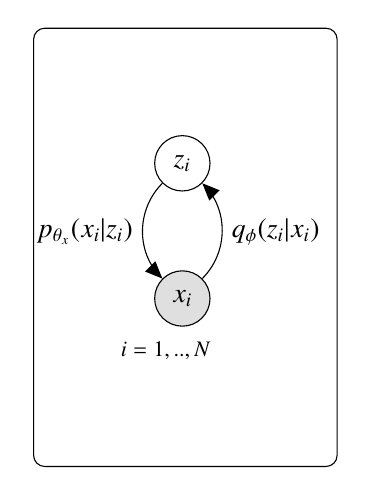
\begin{tikzpicture}
%nodes
\node[latent]   (z)     {$z_i$};
\node[obs, below= of z]       (x) {$x_i$};
% edges
\path[->] (z) edge [bend left=-45] node[mid left] {$p_{\theta_x}(x_i\vert z_i)$} (x)
            (x) edge [bend left=-45] node[mid right] {$q_{\phi}(z_i\vert x_i)$} (z);

\plate [inner sep = 1.35cm, xshift=0.25cm] {plate1} { %
    (x)%
    (z)%
  } {$i=1,..,N$}; %
\end{tikzpicture}
\caption{Vanilla VAE}
\label{fig:vanilla_vae}
\end{center}
\end{figure}

The log likelihood of the data is:
\begin{align*}
    \log{p_{\theta}(x)} = \log{\frac{p(x,z)}{p(z\vert x)}}
\end{align*}

Multiplying both sides by $q_\phi(z \vert x)$ and integrating over $dz$ leads to:
\begin{align*}
    \log{p_{\theta}(x)} &= \int q_\phi(z \vert x) \log{\frac{p_\theta(x,z)}{p(z\vert x)}}dz \\
    &= \int q_\phi(z\vert x) \log{\frac{p_\theta(x,z)}{q_\phi(z\vert x)}\frac{q_\phi(z \vert x)}{p(z \vert x)}}dz \\
    &= \mathbb{E}_{q_\phi(z \vert x)} \log{\frac{p_\theta(x,z)}{q_\phi(z \vert x)}} + \mathbb{KL}(q_\phi(z \vert x) \vert\vert p(z \vert x)) \\
    &\geq \mathbb{E}_{q_\phi(z \vert x)} \log{\frac{p_\theta(x,z)}{q_\phi(z \vert x)}} = \mathcal{L}(\theta, \phi, X)
\end{align*}

In this setting, the D-separation is obvious and the joint distribution factorizes over $n$:
\begin{align*}
    p_{\theta}(x,z) &= \prod_{i=1}^n p_{\theta_x}(x_i \vert z_i) p_{\theta_z}(z_i) \\
    q_{\phi}(z \vert x) &= \prod_{i=1}^n q_{\phi}(z_i \vert x_i)
\end{align*}
The \gls{vlb} (or \gls{elbo}) $\mathcal{L}(\theta, \phi, X)$ simplifies into:
\begin{align*}
    \mathcal{L}(\theta, \phi, X) &= \mathbb{E}_{q_{\phi}(z \vert x)} \log{\frac{\prod_{i=1}^n p_{\theta_x}(x_i \vert z_i) p_{\theta_z}(z_i)}{\prod_{i=1}^n q_{\phi}(z_i \vert x_i)}} \\
    &= \sum_{i=1}^n \mathbb{E}_{q_{\phi}(z_i \vert x_i)} p_{\theta_x}(x_i \vert z_i) - \sum_{i=1}^n \mathbb{KL}(q_{\phi}(z_i \vert x_i) \vert\vert p_{\theta_z}(z_i) )
\end{align*}
The first term is the reconstruction loss, and is estimated via Monte Carlo sampling over $z_i \sim q_{\phi}(z_i \vert x_i)$. The second term is a KL-divergence, which can be computed analytically when $q_\phi$ and $p_{\theta_z}$ are chosen to be Gaussians.

% ---- CODE DE LILIAN ---------------------------------------
% \begin{figure}[H]
% \centering
% \begin{tikzpicture}

% % Nodes
% \node[const] (alpha) {$\alpha$};
% \node[latent, right=of alpha, xshift=1.5cm] (pi) {$\pi$};
% \node[latent, below=of pi, yshift=-1.5cm] (zi) {$z_i$};
% \node[obs, below=of zi, yshift=-1.5cm] (xi) {$x_i$};
% \node[const, left=of xi, yshift=0.5cm, xshift=-1.5cm] (mu) {$\mu$};
% \node[const, left=of xi, yshift=-0.5cm, xshift=-1.5cm] (sigma) {$\Sigma$};


% % Plates
% \plate [inner sep=0.3cm, xshift=0cm, yshift=0cm] {plate1} {(zi)(xi)} {$N$};

% % Edges
% \edge {alpha} {pi};
% \edge {mu, sigma} {xi};
% % \edge {pi} {zi};
% % \edge {zi} {xi};

% % Variational Arrows (dashed arrows for q distributions)
% \path [->] (pi) edge [bend right] node[left] {$p(z | \pi)$} (zi);
% \path [->] (zi) edge [bend right] node[right] {$q_{\phi}(\pi | z)$} (pi);

% \path [->] (zi) edge [bend right] node[left] {$p(x | z)$} (xi);
% \path [->] (xi) edge [bend right] node[right] {$q_{\phi}(z | x)$} (zi);


% \end{tikzpicture}
% \caption{Markovian Hierarchical VAE}
% \label{fig:graphical_variational}
% \end{figure}


%---------------------------------------------------------------------
%--- GAUSSIAN PROCESS 
%---------------------------------------------------------------------

\chapter{Gaussian Process}\label{sec:Gaussian Process}

We summarize here most of the results of the Gaussian Process, and refers the reader to \cite{rasmussen_gaussian_2008} for further details.

We first recall the Gaussian marginal and conditional result:

Let $x$ and $y$ be jointly Gaussian vectors, ie:
\begin{align}
    \begin{bmatrix}
        x \\ y
    \end{bmatrix} &\sim \mathcal{N} \left( 
    \begin{bmatrix}
        \mu_x \\ \mu_y
    \end{bmatrix},
        \begin{bmatrix}
            A & C \\
            C^T & B
        \end{bmatrix}
    \right) = \mathcal{N} \left( 
        \begin{bmatrix}
        \mu_x \\ \mu_y
    \end{bmatrix},
        \begin{bmatrix}
            \tilde{A} & \tilde{C} \\
            \tilde{C}^T & \tilde{B}
        \end{bmatrix}^{-1}
    \right)
\end{align}
where $A, B, C$ is the block decomposition of the covariance matrix, and $\tilde{A}, \tilde{B}, \tilde{C}$ the block decomposition of the precision matrix.

Then the marginal distribution of $x$ and the conditional distribution of $x$ given $y$ are :
\begin{align}
    x &\sim \mathcal{N}(\mu_x, A) \\
    x \vert y &\sim \mathcal{N}(\mu_x + CB^{-1}(y-\mu_y), A-CB^{-1}C^T) \\
    &= \mathcal{N}(\mu_x - \tilde{A}^{-1}\tilde{C}(y-\mu_y), \tilde{A}^{-1})
\end{align}

We now consider a Gaussian Process with mean function $m(.)$ and kernel $k(.,.)$
\begin{align}
    f(x) \sim \mathcal{GP}(m(x), k(x,x'))
\end{align}
At the training points $X = \{x_1,...,x_n\}$, the observations are $Y=\{y_1,...,y_n\}$ with some noise $y = f(x) + \epsilon$ with $\epsilon \overset{i.i.d}{\sim} \mathcal{N}(0,\sigma_n^2)$.

The covariance between observations writes:
\begin{align}
    \text{cov}(y_p,y_q) &= k(x_p, x_q) + \delta_{pd}\sigma_n^2 \\
    \text{cov}(y) &= K(X,X) + \sigma_n^2 I
\end{align}

At some test points $X_*$, we aim to predict $f_* = f(X_*)$. Then:
\begin{align}
    \begin{bmatrix}
        y \\ f_*
    \end{bmatrix} \sim \mathcal{N} \left( 0, \begin{bmatrix}
        K(X,X)+\sigma_n^2I & K(X,X_*) \\ K(X_*,X) & K(X_*,X_*)
    \end{bmatrix}\right)
\end{align}

From which we get:
\begin{align}
    f_* \vert X_*, X, Y &\sim \mathcal{N}(\overline{f_*}, \rm{cov(f_*)}) \\
    \overline{f_*} &= K(X_*,X) \left( K(X,X) + \sigma_n^2 I\right)^{-1}Y \\
    \rm{cov}(f_*) &= K(X_*,X_*) - K(X_*,X) \left( K(X,X) + \sigma_n^2I\right)^{-1} K(X,X_*)
\end{align}


\chapter{KL divergence between two exponential-family distributions}\label{sec:KL-two-exponential-family-distributions}

We recall the family of distributions parameterized by $\eta \in \R^K$, over a fixed support $\mathcal{X}^D \in \R^D$ : the \textbf{exponential family} of distributions $p(x \vert \eta)$ is given by:
\begin{align}
    p(x \vert \eta) &= \frac{1}{Z(\eta)} h(x) \exp\left(\eta^T \mathcal{T}(x)\right) \\
    &= h(x) \exp \left( \eta^T \mathcal{T}(x) - A(\eta)\right)
\end{align}
with:
\begin{itemize}
    \item $h(x)$ is the base measure, ie a scaling constant (often 1)
    \item $\mathcal{T}(x)$ are the sufficient statistics
    \item $\eta$ are the natural parameters, or canonical parameters
    \item $Z(\eta)$ is the partition function, $A(\eta)$ is the log partition function.
\end{itemize}

The Bernoulli, categorical (ie multinomial for one observation), Gaussian distributions are part of the exponential family.

The \textbf{$\mathbb{KL}$-divergence between two exponential family distributions of the same family} is:

\begin{align}
    \mathbb{KL}(p(x\vert \eta_1) \vert \vert p(x \vert \eta_2)) &= \mathbb{E}_{\eta_1}\left[ (\eta_1 - \eta_2) \mathcal{T}(x) - A(\eta_1) + A(\eta_2)\right] \\
    &= (\eta_1 - \eta_2)^T \mathbb{E}_{\eta_1}\mathcal{T}(x) - A(\eta_1) + A(\eta_2)
\end{align}

The most important example is the $\mathbb{KL}$-divergence between two multivariate Gaussian distributions of dimension $D$:

\begin{tcolorbox}[colback=blue!5!white,colframe=black!75!black,title=KL between two multivariate Gaussians of dimension $D$]
\begin{align}
    \label{KL-two-gaussians}
    \mathbb{KL}(\mathcal{N}(x \vert \mu_1, \Sigma_1) \vert\vert \mathcal{N}(x \vert \mu_2, \Sigma_2) &=
    \frac{1}{2}\left[ \text{tr}(\Sigma_2^{-1}\Sigma_1) + (\mu_2-\mu_1)^T \Sigma_2^{-1}(\mu_2-\mu_1) -D + \log{\frac{\vert \Sigma_2\vert}{\vert \Sigma_1 \vert}}\right]
\end{align}
\end{tcolorbox} 
\end{appendices}

\clearpage

\printglossary
\clearpage

%%%%%%%%%%%%%%%%%%%%%%%%%%%%%%%%%%%%%%%%%%%%%%%%%%%%%%%%%%%%%%%%%%%%%%%%%%%%%

\printbibliography
\clearpage

\end{document}